% ===========================================================================
% SOP — 22 Constance St Unit Trust
% Monthly Reporting Pack
% Version 2.0 — March 2026
% ===========================================================================
\documentclass[10pt,a4paper]{article}

% --- Fonts ---
\usepackage[T1]{fontenc}
\usepackage[utf8]{inputenc}
\usepackage{palatino}
\usepackage{mathpazo}
\usepackage[scaled=0.92]{helvet}
\usepackage[protrusion=true,expansion=true,tracking=true,kerning=true,final]{microtype}
\usepackage{setspace}

% --- Layout ---
\usepackage[top=2.2cm, bottom=2.2cm, left=2.2cm, right=2.2cm, headheight=26pt]{geometry}
\setstretch{1.12}

% --- Structure ---
\usepackage{titlesec}
\usepackage{enumitem}
\usepackage{parskip}

% --- Tables ---
\usepackage{booktabs}
\usepackage{tabularx}
\usepackage{array}
\usepackage{multirow}
\usepackage{float}
\usepackage{caption}
\usepackage{longtable}
\usepackage{colortbl}

% --- Visual ---
\usepackage{xcolor}
\usepackage{tcolorbox}
\tcbuselibrary{skins, breakable}
\usepackage{fancyhdr}
\usepackage{lastpage}
\usepackage{graphicx}

% ============================================================
% COMPANY LOGO — replace the filename below with your image
% Supported formats: PDF, PNG, JPG (PDF recommended for best
% print quality). Place the file in the same folder as this
% .tex file, or provide the full path.
%
%   TO USE:  \companylogo            → renders the logo
%   TO SWAP: change "company_logo"   → your actual filename
%            change height=0.65cm    → adjust size as needed
% ============================================================
\newcommand{\companylogo}{%
  \IfFileExists{company_logo.pdf}{%
    \includegraphics[height=0.65cm]{company_logo.pdf}%
  }{\IfFileExists{company_logo.png}{%
    \includegraphics[height=0.65cm]{company_logo.png}%
  }{\IfFileExists{company_logo.jpg}{%
    \includegraphics[height=0.65cm]{company_logo.jpg}%
  }{%
    % ── Fallback: text placeholder when no logo file is found ──
    \small\sffamily\textcolor{navy}{\textbf{22 Constance St Unit Trust}}%
  }}}%
}

\usepackage{amsmath,amssymb}
\usepackage{ragged2e}
\usepackage{calc}
\usepackage{hyperref}
\usepackage{tikz}
\usetikzlibrary{shapes.geometric, shapes.symbols, arrows.meta, positioning, fit, backgrounds, calc}
\pgfdeclarelayer{arrows}
\pgfsetlayers{background,arrows,main}
\usepackage{pdflscape}
\makeatletter
\def\LS@makecol{\setbox\@outputbox\vbox{\pagestyle{fancy}\box\@outputbox}}
\makeatother
\usepackage{rotating}

% ===========================
% COLOUR PALETTE
% ===========================
\definecolor{navy}{HTML}{0F2240}
\definecolor{steel}{HTML}{2C5F8A}
\definecolor{steellight}{HTML}{4A82B0}
\definecolor{sky}{HTML}{C8DDF0}
\definecolor{palesky}{HTML}{E8F2FA}
\definecolor{warmgray}{HTML}{F5F4F2}
\definecolor{midgray}{HTML}{D2D2D2}
\definecolor{lightgray}{HTML}{EBEBEB}
\definecolor{textgray}{HTML}{4A4A4A}
\definecolor{gold}{HTML}{C49A00}
\definecolor{goldbg}{HTML}{FDF8E6}
\definecolor{critred}{HTML}{A82020}
\definecolor{critbg}{HTML}{FDF0F0}
\definecolor{critleft}{HTML}{C62828}
\definecolor{warnamber}{HTML}{B86E00}
\definecolor{warnbg}{HTML}{FEF8ED}
\definecolor{infoteal}{HTML}{167A6A}
\definecolor{infobg}{HTML}{EAF7F4}
\definecolor{contraborder}{HTML}{C49A00}
\definecolor{contrabg}{HTML}{FFF8E7}
\definecolor{tipgreen}{HTML}{276128}
\definecolor{tipbg}{HTML}{F0F8E8}

% ===========================
% HYPERREF
% ===========================
\hypersetup{
    colorlinks=true, linkcolor=steel, urlcolor=steel,
    pdftitle={SOP — 22 Constance St Unit Trust},
    pdfauthor={UFS Fund Accounting},
}

% ===========================
% SECTION HEADINGS
% ===========================
\titleformat{\section}
    {\Large\sffamily\bfseries\color{navy}}
    {\colorbox{navy}{\textcolor{white}{\hspace{3pt}\thesection\hspace{3pt}}}}{0.7em}{}
    [\vspace{2pt}{\color{gold}\rule{\textwidth}{1.2pt}}\vspace{-4pt}]
\titleformat{\subsection}
    {\large\sffamily\bfseries\color{navy}}
    {\textcolor{steel}{\rule[-2pt]{3pt}{12pt}}\hspace{5pt}\textcolor{steel}{\thesubsection}}{0.5em}{}
\titleformat{\subsubsection}
    {\normalsize\sffamily\bfseries\color{steel}}
    {\textcolor{steellight}{\rule[-1pt]{2pt}{9pt}}\hspace{4pt}\textcolor{steellight}{\thesubsubsection}}{0.4em}{}
\titlespacing*{\section}{0pt}{2.0em}{0.9em}
\titlespacing*{\subsection}{0pt}{1.3em}{0.5em}
\titlespacing*{\subsubsection}{0pt}{0.9em}{0.3em}

% ===========================
% HEADER / FOOTER
% ===========================
\pagestyle{fancy}
\fancyhf{}
\fancyhead[L]{\small\sffamily\textcolor{navy}{\textbf{22 Constance St Unit Trust}}}
\fancyhead[R]{\small\sffamily\textcolor{textgray}{SOP \textbullet{} v2.0}}
\fancyfoot[L]{\small\sffamily\textcolor{textgray}{Confidential \textbullet{} Internal Use Only}}
\fancyfoot[C]{\small\sffamily\textcolor{gold}{\rule{1.5cm}{0.4pt}\hspace{4pt}\textbf{\thepage\ of \pageref{LastPage}}\hspace{4pt}\rule{1.5cm}{0.4pt}}}
\fancyfoot[R]{\small\sffamily\textcolor{textgray}{March 2026}}
\renewcommand{\headrulewidth}{0pt}
\renewcommand{\footrulewidth}{0pt}
\renewcommand{\headrule}{%
  \vspace{-2pt}%
  \hbox to\headwidth{\color{navy}\leaders\hrule height 1.4pt\hfill}%
  \vspace{1.5pt}%
  \hbox to\headwidth{\color{gold}\leaders\hrule height 0.5pt\hfill}%
}
\setlength{\headheight}{31.2pt}
\addtolength{\topmargin}{-3.2pt}

% ===========================
% CALLOUT BOXES
% ===========================
\newtcolorbox{critical}[1][]{
    enhanced, breakable, colback=critbg, colframe=critleft,
    boxrule=0pt, leftrule=5pt, borderline north={1pt}{0pt}{critleft!40!white},
    drop shadow southeast,
    fonttitle=\sffamily\bfseries\small\color{white},
    title={\raisebox{-0.5pt}{\textbf{!}}\enspace CRITICAL\ifx&#1&\else\textcolor{white!70!critleft}{\enspace\textbf{·}}\enspace #1\fi},
    attach boxed title to top left={xshift=8pt, yshift=-\tcboxedtitleheight/2},
    boxed title style={colback=critleft, colframe=critleft, rounded corners=all, left=6pt, right=6pt, top=2pt, bottom=2pt},
    top=14pt, bottom=6pt, left=8pt, right=8pt, before skip=22pt, after skip=8pt, rounded corners=south}

\newtcolorbox{warning}[1][]{
    enhanced, breakable, colback=warnbg, colframe=warnamber,
    boxrule=0pt, leftrule=5pt, borderline north={1pt}{0pt}{warnamber!40!white},
    drop shadow southeast,
    fonttitle=\sffamily\bfseries\small\color{white},
    title={$\blacktriangleright$\enspace WARNING\ifx&#1&\else\textcolor{white!70!warnamber}{\enspace\textbf{·}}\enspace #1\fi},
    attach boxed title to top left={xshift=8pt, yshift=-\tcboxedtitleheight/2},
    boxed title style={colback=warnamber, colframe=warnamber, rounded corners=all, left=6pt, right=6pt, top=2pt, bottom=2pt},
    top=14pt, bottom=6pt, left=8pt, right=8pt, before skip=22pt, after skip=8pt, rounded corners=south}

\newtcolorbox{note}[1][]{
    enhanced, breakable, colback=infobg, colframe=infoteal,
    boxrule=0pt, leftrule=5pt, borderline north={1pt}{0pt}{infoteal!35!white},
    drop shadow southeast,
    fonttitle=\sffamily\bfseries\small\color{white},
    title={\textbf{i}\enspace NOTE\ifx&#1&\else\textcolor{white!70!infoteal}{\enspace\textbf{·}}\enspace #1\fi},
    attach boxed title to top left={xshift=8pt, yshift=-\tcboxedtitleheight/2},
    boxed title style={colback=infoteal, colframe=infoteal, rounded corners=all, left=6pt, right=6pt, top=2pt, bottom=2pt},
    top=14pt, bottom=6pt, left=8pt, right=8pt, before skip=22pt, after skip=8pt, rounded corners=south}

% ===========================
% COLUMN TYPES & COMMANDS
% ===========================
\newcolumntype{L}[1]{>{\raggedright\arraybackslash}p{#1}}
\newcolumntype{R}[1]{>{\raggedleft\arraybackslash}p{#1}}
\newcolumntype{C}[1]{>{\centering\arraybackslash}p{#1}}
\newcommand{\thead}[1]{\cellcolor{navy}\textcolor{white}{\sffamily\bfseries\small #1}}
\newcommand{\issuehdr}[2]{\rowcolor{navy}\textcolor{white}{\sffamily\bfseries\small #1} & \textcolor{white}{\sffamily\bfseries\small #2} \\}
\newcommand{\icat}[1]{{\sffamily\scriptsize\textcolor{steel}{#1}}}
\newcommand{\acct}[1]{\mbox{\colorbox{sky!45}{\strut\,\textsf{\textbf{\small #1}}\,}}}
\usepackage{pifont}
\newcommand{\xmark}{\textcolor{critleft}{\ding{55}}}

% Phase banner
\newtcolorbox{phasebox}[2]{
    enhanced, colback=#1!8!white, colframe=#1,
    boxrule=0pt, leftrule=5pt, borderline south={1pt}{0pt}{#1!30!white},
    sharp corners, fontupper=\sffamily\small,
    left=8pt, right=8pt, top=5pt, bottom=4pt, before skip=10pt, after skip=5pt,
    title={\sffamily\bfseries\normalsize\textcolor{white}{#2}},
    attach boxed title to top left={xshift=6pt, yshift=-\tcboxedtitleheight/2},
    boxed title style={colback=#1, colframe=#1, rounded corners=all, left=6pt, right=6pt, top=2pt, bottom=2pt},
    top=11pt}

% ===========================
% FLOWCHART TikZ STYLES
% ===========================
\tikzset{
  proc/.style={rectangle, rounded corners=4pt, draw=steel, line width=0.9pt, fill=palesky,
    font=\sffamily\fontsize{6.5}{8}\selectfont, minimum width=3.6cm, minimum height=1.2cm,
    align=center, text width=3.4cm, inner sep=3pt},
  proc/cpg/.style={rectangle, rounded corners=4pt, draw=critred!80, line width=0.9pt, fill=critbg,
    font=\sffamily\fontsize{6.5}{8}\selectfont, minimum width=3.6cm, minimum height=1.2cm,
    align=center, text width=3.4cm, inner sep=3pt},
  proc/rev/.style={rectangle, rounded corners=4pt, draw=infoteal, line width=0.9pt, fill=infobg,
    font=\sffamily\fontsize{6.5}{8}\selectfont, minimum width=3.6cm, minimum height=1.2cm,
    align=center, text width=3.4cm, inner sep=3pt},
  proc/coord/.style={rectangle, rounded corners=4pt, draw=steel, line width=0.9pt, fill=sky,
    font=\sffamily\fontsize{6.5}{8}\selectfont, minimum width=3.6cm, minimum height=1.2cm,
    align=center, text width=3.4cm, inner sep=3pt},
  docn/.style={tape, tape bend top=none, tape bend height=0.18cm,
    draw=steel!50, line width=0.6pt, fill=warmgray,
    font=\sffamily\fontsize{5.5}{7}\selectfont,
    minimum width=3.0cm, minimum height=0.9cm,
    align=center, text width=2.8cm, inner sep=4pt},
  dec/.style={diamond, aspect=2.2, draw=warnamber, line width=0.9pt, fill=warnbg,
    font=\sffamily\fontsize{6.5}{8}\selectfont, minimum width=2.0cm, align=center, inner sep=2pt},
  lbox/.style={rectangle, rounded corners=3pt, draw=textgray, line width=0.6pt, fill=warmgray,
    font=\sffamily\fontsize{5.5}{7}\selectfont, minimum width=2.2cm, minimum height=0.7cm,
    align=center, text width=2.0cm, inner sep=2pt},
  opc/.style={regular polygon, regular polygon sides=5, shape border rotate=180,
    draw=navy, line width=0.9pt, fill=sky, text=navy,
    font=\sffamily\bfseries\normalsize, minimum size=0.8cm, align=center, inner sep=0pt},
  term/.style={rectangle, rounded corners=6pt, fill=navy, text=white,
    font=\sffamily\bfseries\small, minimum width=5cm, minimum height=0.65cm, align=center, inner sep=4pt},
  ar/.style={-Latex, draw=textgray, line width=0.8pt, rounded corners=6pt, shorten >=3pt, shorten <=2pt},
  lb/.style={font=\sffamily\fontsize{6}{7.5}\selectfont, fill=white, inner sep=1pt, text=textgray},
  lanelbl/.style={font=\sffamily\bfseries\footnotesize, text=white, rotate=90, anchor=center},
}
\newcommand{\PN}[4]{%
  {\fontsize{8}{9.5}\selectfont\bfseries\textcolor{navy}{#1}}\\[1pt]%
  {\fontsize{6}{7.5}\selectfont #2}%
}
\newcommand{\DN}[1]{{\fontsize{5.5}{7}\selectfont #1}}

% ============================================================================
\begin{document}

% ============================================================================
% TITLE PAGE
% ============================================================================
\begin{titlepage}
\thispagestyle{empty}

% Full-height left accent stripe via TikZ (behind content)
\begin{tikzpicture}[remember picture, overlay]
  % Deep navy left stripe
  \fill[navy] (current page.north west) rectangle ([xshift=1.1cm]current page.south west);
  % Gold thin inner edge on the stripe
  \fill[gold] ([xshift=1.0cm]current page.north west) rectangle ([xshift=1.1cm]current page.south west);
  % Top banner bar
  \fill[navy!95!black] ([yshift=-0pt]current page.north west) rectangle ([yshift=-1.1cm]current page.north east);
  % Gold under-line on top banner
  \fill[gold] ([yshift=-1.1cm]current page.north west) rectangle ([yshift=-1.18cm]current page.north east);
  % Bottom accent band
  \fill[navy!90!black] ([yshift=1.6cm]current page.south west) rectangle (current page.south east);
  \fill[gold] ([yshift=1.6cm]current page.south west) rectangle ([yshift=1.68cm]current page.south east);
  % --- Decorative geometric accent: corner chevron pattern (lower-right) ---
  \begin{scope}[opacity=0.06]
    \foreach \i in {0,1,...,8} {
      \draw[navy, line width=2.5pt]
        ([xshift={-1.8cm-\i*0.9cm}, yshift={2.2cm}]current page.south east)
        -- ([xshift={-0.3cm}, yshift={2.2cm+\i*0.9cm+1.5cm}]current page.south east);
    }
  \end{scope}
  % --- Subtle corner accent dot cluster (upper-right) ---
  \begin{scope}[opacity=0.04]
    \foreach \x in {0,...,5} {
      \foreach \y in {0,...,3} {
        \fill[navy] ([xshift={-1.5cm-\x*0.5cm}, yshift={-1.8cm-\y*0.5cm}]current page.north east) circle (1.5pt);
      }
    }
  \end{scope}
  % CONFIDENTIAL label in top bar
  \node[anchor=west, text=white, font=\sffamily\small\bfseries, inner sep=0pt]
    at ([xshift=1.5cm, yshift=-0.55cm]current page.north west)
    {CONFIDENTIAL \textbullet{} FOR INTERNAL USE ONLY};
  % Version pill top-right
  \node[anchor=east, fill=gold, text=navy, font=\sffamily\bfseries\footnotesize,
        rounded corners=3pt, inner xsep=7pt, inner ysep=3pt]
    at ([xshift=-0.4cm, yshift=-0.55cm]current page.north east)
    {Version 2.0 \textbullet{} March 2026};
\end{tikzpicture}

\vspace*{0.5cm}
\hspace*{1.6cm}%
\begin{minipage}{\dimexpr\textwidth-1.6cm}

% Logo
\noindent\companylogo\par
\vspace{1.0cm}

% Main title block
\noindent{\fontsize{34}{40}\selectfont\sffamily\bfseries\textcolor{navy}{Standard Operating\\[4pt]Procedure}}\par
\vspace{0.3cm}
\noindent{\fontsize{15}{20}\selectfont\sffamily\textcolor{steellight}{Monthly Reporting Pack Preparation}}\par
\vspace{0.25cm}
\noindent{\sffamily\small\textcolor{textgray}{Comprehensive month-end accounting, reconciliation, and financial reporting procedures}}\par
\vspace{0.7cm}

% Gold rule
\noindent\textcolor{gold}{\rule{9cm}{1.5pt}}\par
\vspace{0.5cm}

% Fund identity
\noindent{\fontsize{14}{18}\selectfont\sffamily\bfseries\textcolor{navy}{22 Constance St Unit Trust}}\par
\vspace{0.1cm}
\noindent{\sffamily\small\textcolor{textgray}{Unlisted Unit Trust \textbullet{} 22--26A Constance Street, Fortitude Valley QLD 4006}}\par
\vspace{0.9cm}

% Fund details table
\renewcommand{\arraystretch}{1.35}
\begin{tabular}{@{}>{\sffamily\bfseries\small\color{navy}}l @{\hspace{1.4em}} >{\sffamily\small}l @{}}
ABN                 & 28 218 694 388 \\
TFN                 & 552 125 429 \\
Constitution Date   & 17 April 2019 \\
Trustee             & 22 Constance St Pty Ltd (wholly owned subsidiary of CPG) \\
Manager             & Centennial Property Group Pty Ltd (CPG), ACN 151 746 977 \\
Accounting Period   & 1 July to 30 June \\
Document Owner      & UFS Fund Accounting Team \\
\end{tabular}

\vspace{0.9cm}

% Key Personnel box — refined
\begin{tcolorbox}[
    enhanced,
    colback=palesky, colframe=steel,
    boxrule=0pt, leftrule=4pt,
    borderline north={0.5pt}{0pt}{steel!30!white},
    sharp corners,
    left=10pt, right=10pt, top=8pt, bottom=8pt,
    title={\sffamily\bfseries\small\color{white}\raisebox{-0.5pt}{\textbullet}\enspace Key Personnel},
    attach boxed title to top left={xshift=8pt, yshift=-\tcboxedtitleheight/2},
    boxed title style={colback=steel, colframe=steel, sharp corners,
      left=5pt, right=5pt, top=2pt, bottom=2pt}
]
\renewcommand{\arraystretch}{1.25}
\begin{tabular}{@{}>{\sffamily\bfseries\small\color{steel}}l @{\hspace{1.2em}} >{\sffamily\small}l @{}}
Preparer (UFS)            & Anthony Tran \\
1st Reviewer (UFS)        & Pantea Asgari \\
2nd Reviewer (UFS)        & Sonya Beatriz \\
Client Coordinator (UFS)  & Kim Tran \\
Client Contact (CPG)      & William Cassimatis --- wcassimatis@centennial.com.au \\
Client Contact (CPG)      & Ally Hill --- ahill@centennial.com.au \\
\end{tabular}
\end{tcolorbox}

\end{minipage}

\end{titlepage}
\pagenumbering{arabic}
\setcounter{page}{1}
\tableofcontents
\clearpage

% ============================================================================
% 1. FUND SNAPSHOT
% ============================================================================
\section{Fund Snapshot}
\label{sec:snapshot}

Single-asset Australian property unit trust holding a commercial office at Fortitude Valley, QLD. Put \& Call Option Deed executed; Call Option exercised (\$13.25\,M); binding contract in place. Loan maturity approaching (15~Jun~2026). Monthly reporting process: \S\ref{sec:process}. Classification rules: \S\ref{sec:fivecase}--\ref{sec:grp4}. Key issues: \S\ref{sec:issues}. State obligations: \S\ref{sec:state}. Deductible expense guide: \S\ref{sec:deduct}.

\begin{table}[H]
\centering\small\sffamily
\begin{tabularx}{\textwidth}{@{}>\bfseries L{3.6cm} X@{}}
\rowcolor{navy}\textcolor{white}{\bfseries Attribute} & \textcolor{white}{\bfseries Detail} \\
\midrule
Asset & 22--26 Constance St, Fortitude Valley QLD --- commercial office, 2,592~sqm NLA, 1,539~sqm land, incl.\ 1928 Sub Station \\
\rowcolor{warmgray}
Sale Structure & Put \& Call Option Deed (PCOD); Call Option exercised; contract price \$13.25\,M. Option consideration \$1.325\,M held as liability pending settlement. CGT Event~A1 crystallised on exercise of Call Option. \\
Loan & St George \$5.0\,M @ 1.95\% p.a. --- matures \textbf{15 Jun 2026} \\
\rowcolor{warmgray}
Occupancy & $\sim$26.7\% (692/2,592~sqm). Sony 336~sqm holdover 49\% income; 5Point 200~sqm to Oct~27; Popgun 156~sqm to Dec~26 \\
Insurance & Active cyclone claim \$214k YTD Jan~26 (Steadfast/Vision Re) \\
\rowcolor{warmgray}
Trustee / Admin & Centennial Property Group (CPG) / UFS Fund Accounting \\
Banks & NAB (operations account) \textbullet{} St George (loan + insurance receipts) \\
\rowcolor{warmgray}
Fees & Mgmt 5\% net income (\S\ref{sec:grp4c}); Disposal 1\% GAV (\S\ref{sec:grp4b}); Perf.\ 20\%/40\% above 8\%/15\% IRR (\S\ref{sec:grp4d}) \\
Deferred Sale Costs & \$133,732 deferred on balance sheet while PCOD sale active --- see Group~1c (\S\ref{sec:grp1c}) and Group~3b (\S\ref{sec:grp3b}) \\
\rowcolor{warmgray}
Securities & Bank guarantees: 5Point \$33k, Popgun \$61.6k (to be assigned to purchaser at settlement). Option consideration \$1.325\,M held as balance sheet liability \\
\bottomrule
\end{tabularx}
\end{table}

\begin{critical}[Dual Countdown --- Loan Maturity vs.\ Sale Settlement]
St George matures \textbf{15~Jun~2026}. Every monthly pack must assess: (1)~settlement timeline, (2)~loan reclassification as current, (3)~going concern. Sale price \$13.25\,M exceeds loan \$5.0\,M + costs --- solvent if settlement completes on time.
\end{critical}


% ============================================================================
% 2. MONTHLY REPORTING PROCESS
% ============================================================================
\section{Monthly Reporting Process}
\label{sec:process}

\noindent The monthly reporting cycle runs across three phases and ten steps, spanning from the 20th of the prior month through Business Day~5. Phase~1 covers source document collection and bank reconciliation (\S\ref{sec:fivecase}); Phase~2 covers pack compilation and NAV outputs; Phase~3 covers independent review and distribution to CPG. Process flowcharts are at \S\ref{sec:flowchart}; TB reclassification rules at \S\ref{sec:reclass}.

\begin{phasebox}{steel}{Phase 1 --- Source Documents \& Reconciliation \normalfont\small(20th--BD1)}
Collect source documents, import Yardi TB, reconcile NAB using five-case classification (\S\ref{sec:fivecase}).
\end{phasebox}

{\small\sffamily
\begin{tabularx}{\textwidth}{@{}C{0.5cm} L{1.4cm} X@{}}
\rowcolor{navy}\textcolor{white}{\bfseries\#} & \textcolor{white}{\bfseries Actor} & \textcolor{white}{\bfseries Action} \\
\midrule
\textbf{1} & CPG & Upload St George stmt, invoices, supporting docs to SharePoint \\
\rowcolor{warmgray}
\textbf{2} & UFS Coord. & Download NAB bank stmt; archive to UFS Shared Folder \\
\textbf{3} & Preparer & Import Yardi TB (\texttt{cs4001}+\texttt{22chts}); reconcile NAB TB vs.\ bank stmt per five-case classification (\S\ref{sec:fivecase}); must balance to zero \\
\rowcolor{warmgray}
\textbf{4} & Preparer & Submit bank info request to CPG for unidentified items (Case~4) \\
\textbf{5} & CPG & Respond with invoices, insurance remittances, sale status updates \\
\rowcolor{warmgray}
\textbf{6} & Preparer & Revise Yardi TB per reclassification rules (\S\ref{sec:reclass}); import revised TB into pack \\
\bottomrule
\end{tabularx}}

\begin{phasebox}{infoteal}{Phase 2 --- Pack Compilation \normalfont\small(BD2--BD4)}
Build full pack from imported TB. Steps 7a--7j in sequence.
\end{phasebox}

{\small\sffamily
\begin{tabularx}{\textwidth}{@{}C{0.5cm} L{1.4cm} X@{}}
\rowcolor{navy}\textcolor{white}{\bfseries\#} & \textcolor{white}{\bfseries Actor} & \textcolor{white}{\bfseries Action} \\
\midrule
\textbf{7} & Preparer & (a)~Verify Yardi import: income, receivables, prepayments, opex $\to$ (b)~NAB cut-off Sundry Debtor entries Cases~2--5 (\S\ref{sec:grp1a}) $\to$ (c)~St George interest and line fee amortisation (cash basis, \S\ref{sec:grp1c}) $\to$ (d)~Insurance claim receipts via St George + cyclone capital expenditure via NAB --- never net (\S\ref{sec:grp2c}) $\to$ (e)~Deferred sale costs review --- still active? (\S\ref{sec:grp1c} and \S\ref{sec:grp3b}) $\to$ (f)~Borrowing cost amortisation schedule check (\S\ref{sec:grp2b} and \S\ref{sec:grp3c}) $\to$ (g)~Trust-level accruals check for double-count (\S\ref{sec:grp2a}; \S\ref{sec:grp4}) + operating accruals $\to$ (h)~Distribution workings + CPG intercompany balance $\to$ (i)~IP fair value and loan reclassification flag (\S\ref{sec:issues:acct}) $\to$ (j)~NAV, Dashboard, ICR, unit price \\
\bottomrule
\end{tabularx}}

\begin{phasebox}{tipgreen}{Phase 3 --- Review \& Distribution \normalfont\small(BD4--BD5)}
Dual independent review, CPG distribution, and archiving.
\end{phasebox}

{\small\sffamily
\begin{tabularx}{\textwidth}{@{}C{0.5cm} L{1.4cm} X@{}}
\rowcolor{navy}\textcolor{white}{\bfseries\#} & \textcolor{white}{\bfseries Actor} & \textcolor{white}{\bfseries Action} \\
\midrule
\textbf{8} & Preparer & Submit pack to 1st \& 2nd Reviewer via UFS Shared Folder \\
\rowcolor{warmgray}
\textbf{9} & Reviewers & Independent review $\to$ comments (FIX loop) or sign off checklists (NAV, BAS, Distribution) \\
\textbf{10} & 1st Reviewer & (a)~Send approved NAV pack \& monthly report to CPG; address CPG comments if any (resubmit loop) $\to$ (b)~Archive CPG-approved final pack in UFS Shared Folder as permanent record \\
\bottomrule
\end{tabularx}}


% ============================================================================
% 2.1 PROCESS FLOWCHARTS
% ============================================================================
\subsection{Process Flowcharts}
\label{sec:flowchart}

Each numbered node corresponds to a step in the Monthly Reporting Process (above).
Convention: \textbf{Yes}~= issue found (loop back); \textbf{No}~= clear (proceed).

\vspace{0.4em}
\noindent{\small\sffamily
\begin{tabular}{@{}p{3.2cm} >{\centering\arraybackslash}p{1.0cm} >{\raggedright\arraybackslash}p{9.0cm}@{}}
\toprule
\textbf{Symbol} & \textbf{Icon} & \textbf{Description} \\
\midrule
Action / Step block &
  \raisebox{-0.15cm}{\begin{tikzpicture}[baseline]
    \node[rectangle, rounded corners=3pt, draw=steel, line width=0.7pt, fill=palesky,
          minimum width=0.8cm, minimum height=0.45cm, inner sep=1pt,
          font=\sffamily\fontsize{5}{6}\selectfont] {Step N};
  \end{tikzpicture}} &
  Numbered action by the responsible party. Colour: \colorbox{palesky!40}{\strut\,\textcolor{steel}{\scriptsize\bfseries Preparer}\,}\enspace
  \colorbox{infobg!50}{\strut\,\textcolor{infoteal}{\scriptsize\bfseries Reviewer}\,}\enspace
  \colorbox{critbg!50}{\strut\,\textcolor{critred}{\scriptsize\bfseries CPG}\,}\enspace
  \colorbox{sky!50}{\strut\,\textcolor{steel}{\scriptsize\bfseries Coordinator}\,} \\[4pt]
Document &
  \raisebox{-0.15cm}{\begin{tikzpicture}[baseline]
    \node[tape, tape bend top=none, tape bend height=0.13cm,
          draw=steel!50, line width=0.6pt, fill=warmgray,
          minimum width=0.8cm, minimum height=0.45cm, inner sep=1pt,
          font=\sffamily\fontsize{5}{6}\selectfont] {Doc};
  \end{tikzpicture}} &
  Artefact produced or consumed by the preceding action. Contains source name and tab reference. \\[4pt]
Decision &
  \raisebox{-0.18cm}{\begin{tikzpicture}[baseline]
    \node[diamond, aspect=2, draw=warnamber, line width=0.7pt, fill=warnbg,
          minimum width=0.6cm, minimum height=0.35cm, inner sep=0pt,
          font=\sffamily\fontsize{4}{5}\selectfont] {Y/N};
  \end{tikzpicture}} &
  Gateway: \textbf{Yes}~= issue found $\to$ loop back to fix. \textbf{No}~= clear $\to$ proceed to next step. \\[4pt]
Off-page connector &
  \raisebox{-0.15cm}{\begin{tikzpicture}[baseline]
    \node[regular polygon, regular polygon sides=5, shape border rotate=180,
          draw=navy, line width=0.7pt, fill=sky, text=navy,
          minimum size=0.4cm, inner sep=0pt,
          font=\sffamily\bfseries\fontsize{5.5}{6.5}\selectfont] {A};
  \end{tikzpicture}} &
  Links across flowchart pages. A~$\to$~B~$\to$~C~$\to$~D traces the full process path. \\[4pt]
Sync bar &
  \raisebox{0.02cm}{\begin{tikzpicture}[baseline]
    \node[rectangle, fill=navy, draw=navy,
          minimum width=0.7cm, minimum height=0.08cm, inner sep=0pt] {};
  \end{tikzpicture}} &
  All parallel branches must complete before the process continues past the bar. \\
\bottomrule
\end{tabular}}

\vspace{0.5em}

%  PAGE 1 OF 5 — Phase 1a: Steps 1--3  (Source Documents & Reconciliation)
% ==========================================================================
\begin{landscape}
\vspace*{-0.4cm}
\begin{center}
{\sffamily\bfseries\large\textcolor{navy}{Phase 1a --- Source Document Collection \& Reconciliation (Steps 1--3)}}\par\vspace{0.25cm}

\resizebox{0.96\linewidth}{!}{%
\begin{tikzpicture}[every node/.style={font=\sffamily}]

%% ===== NODES =====
\node[term] (START) at (12,0.5) {BEGIN};

% -- CPG Lane: Step 1 --
\node[proc/cpg] (S1) at (4,-2.5) {\PN{1}{Upload source docs to CPG SharePoint}{CPG}{BD1}};
\node[docn]     (D1) at (11,-2.5) {\DN{St George bank stmt, bank info responses, invoices (remediation, insurance, sale) $\to$ SharePoint}};

% -- Coordinator Lane: Step 2 --
\node[proc]  (S2) at (4,-6.0) {\PN{2}{Download NAB bank stmt; archive in UFS Shared Folder}{Client Coord.}{20th \& BD1}};
\node[docn]  (D2) at (11,-6.0) {\DN{NAB bank stmt $\to$ UFS Shared Folder}};

% -- Preparer Lane: Step 3 --
\node[proc]  (S3) at (4,-10.0) {\PN{3}{Download Yardi TB exports \& StG stmt; reconcile NAB TB vs bank stmt}{Preparer}{20th \& BD1}};
\node[docn]  (D3) at (11,-10.0) {\DN{cs4001, 22chts exports; Yardi vs Bank Stat Rec tab (5 cases)}};
\node[dec]   (R3) at (17,-10.0) {Differences\\remain?};
\node[lbox]  (F3) at (17,-13.0) {Investigate \&\\resolve differences\\{\textit{Preparer}}};

\node[opc] (OB2) at (23,-10.0) {A};
\node[lb, right=0.1cm of OB2] {\textit{Ph.1b: Bank Info \& TB Import}};

\begin{scope}[on background layer]
  \def\LaneStripL{-1.2}
  \def\LaneStripR{0}
  \fill[critred!75] (\LaneStripL, 0.9) rectangle (\LaneStripR,-4.2);
  \fill[steel]      (\LaneStripL,-4.2) rectangle (\LaneStripR,-7.8);
  \fill[steel!65]   (\LaneStripL,-7.8) rectangle (\LaneStripR,-14.5);
  \fill[critbg!35]  (0, 0.9) rectangle (25.5,-4.2);
  \fill[palesky!25] (0,-4.2) rectangle (25.5,-7.8);
  \fill[palesky!12] (0,-7.8) rectangle (25.5,-14.5);
  \node[lanelbl] at (-0.6,-1.65) {CPG};
  \node[lanelbl] at (-0.6,-6.00) {Coordinator};
  \node[lanelbl] at (-0.6,-11.15) {Preparer};
  \draw[midgray, dashed, line width=0.35pt] (\LaneStripL,-4.2) -- (25.5,-4.2);
  \draw[midgray, dashed, line width=0.35pt] (\LaneStripL,-7.8) -- (25.5,-7.8);
\end{scope}

\begin{pgfonlayer}{arrows}
\draw[draw=textgray, line width=0.8pt, rounded corners=6pt] (START.west) -- (0.5,0.5) -- (0.5,-6.0);
\draw[ar] (0.5,-2.5)  -- node[lb,above]{begin} (S1.west);
\draw[ar] (0.5,-6.0)  -- node[lb,above]{begin} (S2.west);
\draw[ar] (S1.east) -- node[lb,above]{upload} (D1.west);
\draw[ar] (S2.east) -- node[lb,above]{archive} (D2.west);
\draw[ar] (D1.east) -- node[lb,above]{feeds} (16,-2.5) -- (16,-8.0) -- (4,-8.0) -- (S3.north);
\draw[ar] (D2.south) -- node[lb,right]{feeds} (11,-7.5) -- (1.5,-7.5) -- (1.5,-10.0) -- (S3.west);
\draw[ar] (S3.east) -- node[lb,above]{reconcile} (D3.west);
\draw[ar] (D3.north) -- node[lb,right]{review} (11,-8.5) -- (17,-8.5) -- (R3.north);
\draw[ar] (R3.east) -- node[lb,above]{No} (OB2.west);
\draw[ar] (R3.south) -- node[lb,right]{Yes} (F3.north);
\draw[ar] (F3.west) -- node[lb,above]{retest} (13.5,-13.0) -- (13.5,-10.0) -- (R3.west);
\end{pgfonlayer}
\end{tikzpicture}
}%
\end{center}
\end{landscape}

% ==========================================================================
%  PAGE 2 OF 5 — Phase 1b: Steps 4--6  (Bank Info Request & TB Import)
% ==========================================================================
\begin{landscape}
\vspace*{-0.4cm}
\begin{center}
{\sffamily\bfseries\large\textcolor{navy}{Phase 1b --- Bank Information Request \& TB Import (Steps 4--6)}}\par\vspace{0.25cm}

\resizebox{0.96\linewidth}{!}{%
\begin{tikzpicture}[every node/.style={font=\sffamily}]

\node[opc] (OA) at (1,-2.8) {A};
\node[lb, above=0.1cm of OA] {\textit{from Ph.1a}};

\node[proc] (S4) at (5.5,-2.8) {\PN{4}{Prepare bank info request (Excel)}{Preparer}{20th \& BD1}};
\node[docn] (D4) at (11.5,-2.8) {\DN{Bank info request (Excel) with all queries drafted}};

\node[proc] (S6) at (18,-2.8) {\PN{6}{Revise Yardi TB (reclass trust / sale / leasing); import}{Preparer}{BD1}};
\node[docn] (D6) at (24,-2.8) {\DN{Yardi\_TB revised; Import\_Yardi tab updated}};

\node[opc] (OB) at (24,-6.2) {B};
\node[lb, right=0.1cm of OB] {\textit{Ph.2a: Prop.Level}};

\node[dec]  (R6) at (24,-4.5) {Import\\errors?};
\node[lbox] (F6) at (18,-4.5) {Fix reclassification\\errors\\{\textit{Preparer}}};

\node[proc/coord] (SC) at (5.5,-6.2) {\PN{}{Review bank info request (Excel)}{Coordinator}{BD1}};
\node[dec]  (RC) at (11.5,-6.2) {Review\\notes?};
\node[lbox] (FCN) at (15.0,-6.2) {Return to Preparer\\with review notes};

\node[proc/cpg] (S5) at (5.5,-10) {\PN{5}{Respond to bank info; upload invoices to SharePoint}{CPG}{20th--BD1}};
\node[docn]     (D5) at (12,-10) {\DN{Invoices, remittances, bank info responses $\to$ SharePoint}};
\node[dec]      (R5) at (20,-10) {Outstanding\\items?};
\node[lbox]     (F5) at (25,-10) {Follow up with\\CPG for\\outstanding items};

\begin{scope}[on background layer]
  \fill[palesky!20]  (0,-1.3) rectangle (26.5,-4.2);
  \fill[sky!30]      (0,-4.2) rectangle (26.5,-8.0);
  \fill[critbg!35]   (0,-8.0) rectangle (26.5,-11.8);
  \node[lanelbl, fill=steel!65, minimum width=2.9cm, minimum height=0.85cm,
        rounded corners=2pt] at (-0.7,-2.75) {Preparer};
  \node[lanelbl, fill=steel, minimum width=3.8cm, minimum height=0.85cm,
        rounded corners=2pt] at (-0.7,-6.1) {Coordinator};
  \node[lanelbl, fill=critred!75, minimum width=3.8cm, minimum height=0.85cm,
        rounded corners=2pt] at (-0.7,-9.9) {CPG};
  \draw[midgray, dashed, line width=0.35pt] (0,-4.2)  -- (26.5,-4.2);
  \draw[midgray, dashed, line width=0.35pt] (0,-8.0)  -- (26.5,-8.0);
  \draw[steel!30, dashed, line width=0.35pt] (15,-1.3) -- (15,-4.2);
\end{scope}

\begin{pgfonlayer}{arrows}
\draw[ar] (OA.east) -- node[lb,above]{enter} (S4.west);
\draw[ar] (S4.east) -- node[lb,above]{draft} (D4.west);
\draw[ar] (D4.south) -- node[lb,right]{submit} (11.5,-4.2) -- (5.5,-4.2) -- (SC.north);
\draw[ar] (SC.east) -- node[lb,above]{check} (RC.west);
\draw[ar] (RC.east) -- node[lb,above]{Yes} (FCN.west);
\draw[ar] (RC.south) -- node[lb,right]{No} (11.5,-8.0) -- (5.5,-8.0) -- (S5.north);
\draw[ar] (S5.east) -- node[lb,above]{respond} (D5.west);
\draw[ar] (D5.east) -- node[lb,above]{review} (R5.west);
\draw[ar] (R5.east) -- node[lb,above]{Yes} (F5.west);
\draw[ar] (F5.south) -- node[lb,below]{chase} (25,-11.5) -- (5.5,-11.5) -- (S5.south);
\draw[ar] (R5.north) -- node[lb,right]{No} (20,-8.2) -- (26.5,-8.2) -- (26.5,-1.6) -- (18,-1.6) -- (S6.north);
\draw[ar] (S6.east) -- node[lb,above]{import} (D6.west);
\draw[ar] (D6.south) -- node[lb,right]{review} (R6.north);
\draw[ar] (R6.west) -- node[lb,above]{Yes} (F6.east);
\draw[ar] (F6.north) -- node[lb,right]{redo} (S6.south);
\draw[ar] (R6.south) -- node[lb,right]{No} (OB.north);
\draw[ar] (FCN.north) -- node[lb,above]{revise} (15.0,-1.0) -- (5.5,-1.0) -- (S4.north);
\end{pgfonlayer}

\end{tikzpicture}
}%
\end{center}
\end{landscape}

% ==========================================================================
%  PAGE 3 OF 5 — Phase 2a: Step 7 Sub-steps a--e (Property-Level Entries)
% ==========================================================================
\begin{landscape}
\vspace*{-0.4cm}
\begin{center}
{\sffamily\bfseries\large\textcolor{navy}{Phase 2a --- Reporting Pack Compilation: Property-Level (Steps 7a--7e)}}\par\vspace{0.25cm}

\resizebox{0.96\linewidth}{!}{%
\begin{tikzpicture}[every node/.style={font=\sffamily}]

\node[opc] (OB) at (1,-2) {B};
\node[lb, above=0.1cm of OB] {\textit{from Ph.1b}};

\node[proc] (S7a) at (6,-2) {\PN{7a}{Record property-level entries (Categories A / B / C)}{Preparer}{BD2}};
\node[docn] (D7a) at (13,-2) {\DN{Import\_Yardi, Receivables, Cash, Prepayments tabs verified}};
\node[proc] (S7b) at (19,-2) {\PN{7b}{NAB cut-off Sundry Debtor entries (Cases 2--5)}{Preparer}{BD2}};
\node[docn] (D7b) at (24.5,-2) {\DN{Yardi vs Bank Rec tab; Sundry Debtor journals posted}};
\node[dec]  (R7b) at (24.5,-4.5) {Unmatched\\items?};
\node[lbox] (F7b) at (19,-4.5) {Resolve unmatched\\items; re-check\\5-case coding};

\node[proc] (S7c) at (6,-6.5) {\PN{7c}{Record StG interest (303.01) \& line fee (303.02) --- cash basis}{Preparer}{BD2--3}};
\node[docn] (D7c) at (13,-6.5) {\DN{Loan\_StG tab; StG bank stmt from SharePoint}};

\node[proc] (S7d) at (6,-9.5) {\PN{7d}{Insurance claim income (73.02); cyclone capex (781.01)}{Preparer}{BD3}};
\node[docn] (D7d) at (13,-9.5) {\DN{Capex tab; StG stmt (claim receipts); NAB stmt (capex pmts)}};
\node[dec]  (R7d) at (19,-9.5) {FV update\\needed?};
\node[lbox] (F7d) at (19,-11.8) {Update carrying\\value to valuation\\+ post-val capex};

\node[proc] (S7e) at (6,-13.5) {\PN{7e}{Update deferred cost of sale (709) from new invoices}{Preparer}{BD3}};
\node[docn] (D7e) at (13,-13.5) {\DN{Receivables tab; SharePoint / Yardi sale invoices}};

\node[opc] (OC) at (25,-9.5) {C};
\node[lb, right=0.1cm of OC] {\textit{Ph.2b: Trust-Level}};

\begin{scope}[on background layer]
  \fill[palesky!20] (0,-0.5) rectangle (27,-15);
  \node[lanelbl, fill=steel!65, minimum width=14.5cm, minimum height=0.85cm,
        rounded corners=2pt] at (-0.7,-7.75) {\textcolor{white}{Preparer --- Step 7 Compilation (Property-Level: 7a--7e)}};
  \draw[midgray, dashed, line width=0.35pt] (0,-5.0)  -- (27,-5.0);
  \draw[midgray, dashed, line width=0.35pt] (0,-8.2)  -- (27,-8.2);
  \draw[midgray, dashed, line width=0.35pt] (0,-12.0) -- (27,-12.0);
\end{scope}

\begin{pgfonlayer}{arrows}
\draw[ar] (OB.east) -- node[lb,above]{parallel} (S7a.west);

\coordinate (spC) at (1.0,-6.5);
\coordinate (spD) at (1.0,-9.5);
\coordinate (spE) at (1.0,-13.5);

\draw[draw=textgray, line width=0.8pt, rounded corners=6pt] (OB.south) -- (spE);
\draw[ar] (spC) -- node[lb,above]{parallel} (S7c.west);
\draw[ar] (spD) -- node[lb,above]{parallel} (S7d.west);
\draw[ar] (spE) -- node[lb,above]{parallel} (S7e.west);

\draw[ar] (S7a.east) -- node[lb,above]{verify} (D7a.west);
\draw[ar] (D7a.east) -- node[lb,above]{feeds}  (S7b.west);
\draw[ar] (S7b.east) -- node[lb,above]{post} (D7b.west);
\draw[ar] (D7b.south) -- node[lb,right]{review} (R7b.north);
\draw[ar] (R7b.west) -- node[lb,above]{Yes} (F7b.east);
\draw[ar] (F7b.north) -- node[lb,right]{redo} (S7b.south);
\draw[ar] (R7b.south) -- node[lb,right]{No} (24.5,-8.1) -- (25.4,-8.1) -- (OC.north east);

\draw[ar] (S7c.east) -- node[lb,above]{record} (D7c.west);
\draw[ar] (D7c.east) -- node[lb,above]{done} (22.0,-6.5) -- (22.0,-8.5) -- (OC.north west);

\draw[ar] (S7d.east) -- node[lb,above]{capitalise} (D7d.west);
\draw[ar] (D7d.east) -- node[lb,above]{review} (R7d.west);
\draw[ar] (R7d.south) -- node[lb,right]{Yes} (F7d.north);
\draw[ar] (F7d.west) -- node[lb,above]{redo} (6,-11.8) -- (S7d.south);
\draw[ar] (R7d.east) -- node[lb,above]{No} (OC.west);

\draw[ar] (S7e.east) -- node[lb,above]{update} (D7e.west);
\draw[ar] (D7e.east) -- node[lb,right]{done} (22.0,-13.5) -- (22.0,-10.5) -- (OC.south west);
\end{pgfonlayer}
\end{tikzpicture}
}%
\end{center}
\end{landscape}

% ==========================================================================
%  PAGE 4 OF 5 — Phase 2b: Step 7 Sub-steps f--j (Trust-Level & Outputs)
% ==========================================================================
\begin{landscape}
\vspace*{-0.4cm}
\begin{center}
{\sffamily\bfseries\large\textcolor{navy}{Phase 2b --- Reporting Pack Compilation: Trust-Level \& Outputs (Steps 7f--7j)}}\par\vspace{0.25cm}

\resizebox{!}{0.80\textheight}{%
\begin{tikzpicture}[every node/.style={font=\sffamily}]

\node[opc] (OC) at (1,-1.5) {C};
\node[lb, above=0.1cm of OC] {\textit{from Ph.2a}};

\node[proc] (S7f) at (6,-1.5)  {\PN{7f}{Borrowing cost amortisation (303.03, 303.04)}{Preparer}{BD3}};
\node[docn] (D7f) at (13,-1.5) {\DN{Borrowing cost prepaid tab; straight-line schedule}};

\node[proc] (S7g) at (6,-4.6)  {\PN{7g}{Trust-level accruals (882.16) \& operating accruals (882.02)}{Preparer}{BD3}};
\node[docn] (D7g) at (13,-4.6) {\DN{Accruals tab; CPG invoices; contracts; prior-period patterns}};
\node[dec]  (R7g) at (19,-4.6) {Support\\missing?};
\node[lbox] (F7g) at (19,-6.4) {Obtain missing\\invoices / CPG\\confirmation};

\node[proc] (S7h) at (6,-7.7)  {\PN{7h}{Inter-group loan (882.08) \& distribution payable (882.03)}{Preparer}{BD3}};
\node[docn] (D7h) at (13,-7.7) {\DN{Unitholders tab; CPG written approval for distribution}};

\node[proc] (S7i) at (6,-10.8)  {\PN{7i}{Lease review, IP book value check, loan maturity flag}{Preparer}{BD4}};
\node[docn] (D7i) at (13,-10.8) {\DN{Lease schedule; Capex tab (IP vs valuation); StG maturity flag}};
\node[dec]  (SR)  at (19,-10.8) {Self-review:\\gaps found?};
\node[lbox] (FSR) at (19,-12.6) {Identify gaps \&\\complete entries\\{\textit{Preparer}}};

\node[rectangle, fill=navy, draw=navy, minimum width=6.5cm, minimum height=0.18cm,
      inner sep=0pt] (J7) at (22.75,-13.35) {};
\node[lb, right=0.05cm of J7, font=\sffamily\fontsize{5}{6}\selectfont,
      text=navy] {\textit{sync}};

\node[proc] (S7j) at (6,-14.3)  {\PN{7j}{NAV Statement, Dashboard, ICR, unit price}{Preparer}{BD4}};
\node[docn] (D7j) at (13,-14.3) {\DN{NAV per unit; Dashboard; GL/PL/BS/CFS tabs; OE formula check}};

\node[opc] (OD) at (19,-14.3) {D};
\node[lb, above=0.1cm of OD] {\textit{Ph.3: Review}};

\begin{scope}[on background layer]
  \fill[palesky!20] (0,-0.3) rectangle (26,-15.8);
  \node[lanelbl, fill=steel!65, minimum width=15.8cm, minimum height=0.85cm,
        rounded corners=2pt] at (-0.7,-8.0) {\textcolor{white}{Preparer --- Step 7 Compilation (Trust-Level \& Final Outputs: 7f--7j)}};
  \draw[midgray, dashed, line width=0.35pt] (0,-3.05) -- (26,-3.05);
  \draw[midgray, dashed, line width=0.35pt] (0,-6.15) -- (26,-6.15);
  \draw[midgray, dashed, line width=0.35pt] (0,-9.25) -- (26,-9.25);
  \draw[midgray, dashed, line width=0.35pt] (0,-12.55) -- (26,-12.55);
\end{scope}

\begin{pgfonlayer}{arrows}
\coordinate (BUS2) at (1.0,-4.6);
\coordinate (BUS3) at (1.0,-7.7);
\coordinate (BUS4) at (1.0,-10.8);

\draw[ar] (OC.east) -- node[lb,above]{parallel} (S7f.west);
\draw[draw=textgray, line width=0.8pt, rounded corners=6pt] (OC.south) -- (BUS4);
\draw[ar] (BUS2) -- node[lb,above]{parallel} (S7g.west);
\draw[ar] (BUS3) -- node[lb,above]{parallel} (S7h.west);
\draw[ar] (BUS4) -- node[lb,above]{parallel} (S7i.west);

\draw[ar] (S7f.east) -- node[lb,above]{amortise} (D7f.west);
\draw[ar] (D7f.east) -- node[lb,above]{done} (25.5,-1.5) -- (25.5,-13.35);

\draw[ar] (S7g.east) -- node[lb,above]{post} (D7g.west);
\draw[ar] (D7g.east) -- node[lb,above]{check} (R7g.west);
\draw[ar] (R7g.south) -- node[lb,right]{Yes} (F7g.north);
\draw[ar] (F7g.west) -- node[lb,above]{redo} (6,-6.4) -- (S7g.south);
\draw[ar] (R7g.east) -- node[lb,above]{No} (24.0,-4.6) -- (24.0,-13.35);

\draw[ar] (S7h.east) -- node[lb,above]{record} (D7h.west);
\draw[ar] (D7h.east) -- node[lb,above]{done} (22.5,-7.7) -- (22.5,-13.35);

\draw[ar] (S7i.east) -- node[lb,above]{check} (D7i.west);
\draw[ar] (D7i.east) -- node[lb,above]{review} (SR.west);
\draw[ar] (SR.south) -- node[lb,right]{Yes} (FSR.north);
\draw[ar] (FSR.west) -- node[lb,above]{fix} (6,-12.6) -- (S7i.south);
\draw[ar] (SR.east) -- node[lb,above]{No} (21.0,-10.8) -- (21.0,-13.35);

\draw[ar] (22.75,-13.44) -- node[lb,right]{sync} (22.75,-16.0) -- (6,-16.0) -- (S7j.south);
\draw[ar] (S7j.east) -- node[lb,above]{compile} (D7j.west);
\draw[ar] (D7j.east) -- node[lb,above]{exit} (OD.west);
\end{pgfonlayer}

\end{tikzpicture}
}%
\end{center}
\end{landscape}

% ==========================================================================
%  PAGE 5 OF 5 — Phase 3: Steps 8--10  (Review & Client Distribution)
% ==========================================================================
\begin{landscape}
\vspace*{-0.4cm}
\begin{center}
{\sffamily\bfseries\large\textcolor{navy}{Phase 3 --- Internal Review \& Client Distribution (Steps 8--10)}}\par\vspace{0.25cm}

\resizebox{0.96\linewidth}{!}{%
\begin{tikzpicture}[every node/.style={font=\sffamily}]

\node[opc] (OD) at (1,-3) {D};
\node[lb, above=0.1cm of OD] {\textit{from Ph.2b}};

\node[proc] (S8) at (6,-3) {\PN{8}{Send completed pack to 1st \& 2nd Reviewer}{Preparer}{BD4}};
\node[docn] (D8) at (13,-3) {\DN{Full reporting workbook via UFS Shared Folder}};
\node[lbox] (CLR) at (20,-3) {Preparer clears\\all comments;\\re-submits pack};

\node[proc/rev] (S9)  at (6,-7)    {\PN{9}{Review pack independently; document comments; sign checklists}{1st \& 2nd Reviewer}{BD5}};
\node[dec]      (R9)  at (13,-7)    {Issues\\found?};
\node[lbox]     (FIX) at (20,-7)    {Return to Preparer;\\clear comments \&\\address failed items};
\node[lbox]     (SGN) at (13,-8.8)  {Sign\\Checklist};
\node[docn]     (D9)  at (6,-8.8)   {\DN{NAV checklist, BAS checklist, Distribution checklist signed}};

\node[proc/rev] (S10) at (6,-11.5) {\PN{10a}{Send approved NAV pack \& monthly report to CPG}{1st Reviewer}{BD5}};
\node[docn]     (D10) at (13,-11.5) {\DN{NAV pack, monthly report sent to CPG}};
\node[dec]      (R10) at (18,-11.5) {CPG\\comments?};
\node[lbox]     (RESUB) at (23,-11.5) {Address CPG\\comments; resubmit\\revised pack};
\node[proc, minimum width=3.6cm] (ARC) at (8,-14.5) {\PN{10b}{Archive CPG-approved pack in UFS Shared Folder}{1st Reviewer}{BD5}};
\node[docn] (DARC) at (15,-14.5) {\DN{Final approved pack archived in UFS Shared Folder}};
\node[term, minimum width=4cm] (END) at (15,-16.3) {END};

\begin{scope}[on background layer]
  \fill[palesky!20] (0,-1.8) rectangle (25.5,-5.0);
  \fill[infobg!30]  (0,-5.0) rectangle (25.5,-10.0);
  \fill[critbg!35]  (0,-10.0) rectangle (25.5,-15.2);
  \fill[palesky!5]  (0,-15.2) rectangle (25.5,-16.8);
  \node[lanelbl, fill=steel!65, minimum width=3.2cm, minimum height=0.85cm,
        rounded corners=2pt] at (-0.7,-3.4) {Preparer};
  \node[lanelbl, fill=infoteal, minimum width=5.0cm, minimum height=0.85cm,
        rounded corners=2pt] at (-0.7,-7.5) {1st \& 2nd Reviewer};
  \node[lanelbl, fill=critred!75, minimum width=5.2cm, minimum height=0.85cm,
        rounded corners=2pt] at (-0.7,-12.6) {CPG / Archive};
  \draw[midgray, dashed, line width=0.35pt] (0,-5.0)  -- (25.5,-5.0);
  \draw[midgray, dashed, line width=0.35pt] (0,-10.0) -- (25.5,-10.0);
  \draw[midgray, dashed, line width=0.35pt] (0,-15.2) -- (25.5,-15.2);
\end{scope}

\begin{pgfonlayer}{arrows}
\draw[ar] (OD.east) -- node[lb,above]{enter} (S8.west);
\draw[ar] (S8.east) -- node[lb,above]{submit} (D8.west);
\draw[ar] (D8.south) -- node[lb,right]{assign} (13,-5.2) -- (6,-5.2) -- (S9.north);
\draw[ar] (S9.east) -- node[lb,above]{assess} (R9.west);
\draw[ar] (R9.east) -- node[lb,above]{Yes} (FIX.west);
\draw[ar] (FIX.north) -- node[lb,right]{return} (CLR.south);
\draw[ar] (CLR.north) -- node[lb,above]{resubmit} (20,-1.5) -- (6,-1.5) -- (S8.north);
\draw[ar] (R9.south) -- node[lb,right]{No} (SGN.north);
\draw[ar] (SGN.west) -- node[lb,above]{sign} (D9.east);
\draw[ar] (D9.south) -- node[lb,right]{approve} (S10.north);
\draw[ar] (S10.east) -- node[lb,above]{send} (D10.west);
\draw[ar] (D10.east) -- node[lb,above]{review} (R10.west);
\draw[ar] (R10.east) -- node[lb,above]{Yes} (RESUB.west);
\draw[ar] (RESUB.south) -- node[lb,below]{revise} (23,-13.0) -- (6,-13.0) -- (S10.south);
\draw[ar] (R10.north) -- node[lb,right]{No} (18,-10.6) -- (24.5,-10.6) -- (24.5,-13.6) -- (5.5,-13.6) -- (5.5,-14.5) -- (ARC.west);
\draw[ar] (ARC.east) -- node[lb,above]{archive} (DARC.west);
\draw[ar] (DARC.south) -- node[lb,right]{close} (END.north);
\end{pgfonlayer}
\end{tikzpicture}
}%
\end{center}
\end{landscape}

% ============================================================================
% 2.2  GROUP 1 --- IDENTIFY WHAT IT IS
% ============================================================================
\subsection{Group 1 --- Identify What It Is}
\label{sec:fivecase}

Group~1 covers three classification questions that must be answered before any entry is posted: (1a)~whether a bank timing difference is a Sundry Debtor case; (1b)~whether a property cost is a utility, maintenance, repair, or capital item; and (1c)~which activity bucket --- sale, leasing, operating, or financing --- an identified cost belongs to. All three must be resolved before the cost is posted.

\subsubsection{1a --- Bank Timing: Cash vs.\ Sundry Debtor}
\label{sec:grp1a}

The Yardi ledger and the NAB bank statement are reconciled monthly. Any difference arises from timing only --- not from classification error. Five mutually exclusive cases; the reconciliation must balance to zero.

{\small\sffamily
\begin{longtable}{@{} C{0.7cm} L{3.6cm} p{\dimexpr\textwidth-4.3cm-6\tabcolsep\relax} @{}}
\rowcolor{navy}\textcolor{white}{\bfseries Case} & \textcolor{white}{\bfseries Condition} & \textcolor{white}{\bfseries What to Do} \\
\midrule
\endfirsthead
\rowcolor{navy}\textcolor{white}{\bfseries Case} & \textcolor{white}{\bfseries Condition} & \textcolor{white}{\bfseries What to Do} \\
\midrule
\endhead
\textbf{1} & Yardi and bank agree this month & No action required. \\
\midrule
\rowcolor{warmgray}
\textbf{2} & Yardi recorded last month; bank clears this month & Bank is catching up. Raise a Sundry Debtor entry to bridge the one-month gap. The entry reverses next month when the bank catches up. \\
\midrule
\textbf{3} & Bank processed this month; Yardi records next month & Bank is ahead of Yardi. Raise a Sundry Debtor entry this month and reverse it in Yardi next month. \\
\midrule
\rowcolor{warmgray}
\textbf{4} & Bank item has no matching Yardi entry & Unidentified item. Send a bank information request to CPG (Step~4). Hold in Sundry Debtor until the nature is confirmed: insurance receipt, intercompany transfer, government charge. Do not post to P\&L until confirmed. \\
\midrule
\textbf{5} & Yardi entry has no matching bank item & Yardi is ahead of the bank (a payment raised in Yardi but not yet cleared). Raise a Sundry Debtor entry. If still uncleared after two months, escalate to CPG. \\
\bottomrule
\end{longtable}}

\begin{note}[Test: Which Case Applies?]
Does the item appear in both Yardi \emph{and} the bank this month? $\to$ Case~1, no action. Is it in Yardi only? $\to$ Case~5 (Yardi ahead). Is it in the bank only? $\to$ Case~4 if unidentified, or Case~2 if Yardi recorded it last month. Did the bank clear it before Yardi has recorded it? $\to$ Case~3. The Sundry Debtor entry corrects timing only --- it does not change the underlying expense or income classification.
\end{note}


\subsubsection{1b --- Repair vs.\ Maintenance vs.\ Utilities vs.\ Capital}
\label{sec:capex}

Every invoice for work on the building or its services must be assigned to one of four buckets before posting. The classification determines whether the cost is expensed immediately or capitalised and depreciated. Authority: TR~97/23 (repairs), s25-10 ITAA 1997 (repairs deductible), Div~40 (plant depreciation), Div~43 (building write-off).

{\small\sffamily
\begin{longtable}{@{} L{2.2cm} L{3.2cm} L{7.3cm} @{}}
\rowcolor{navy}
\textcolor{white}{\bfseries Bucket} & \textcolor{white}{\bfseries Definition} & \textcolor{white}{\bfseries Guidance \& Test} \\
\midrule
\endfirsthead
\rowcolor{navy}\textcolor{white}{\bfseries Bucket} & \textcolor{white}{\bfseries Definition} & \textcolor{white}{\bfseries Guidance \& Test} \\
\midrule
\endhead
\textbf{Utilities} & Metered or billed consumption. No physical asset acquired. & \textbf{Test:} Is this billed by a service authority based on consumption or a fixed availability charge (electricity, water, sewerage, gas, waste)? $\to$ Utilities. Expense in the period consumed. If the invoice has not arrived at period end, accrue based on the prior period amount. \\
\rowcolor{warmgray}
\textbf{Maintenance} & Routine, scheduled servicing of an existing asset. Keeps it in its current condition; does not improve it. & \textbf{Test:} Is this periodic, recurring, and triggered by a schedule or contract rather than damage or failure? $\to$ Maintenance. Not triggered by the cyclone or any specific event --- it would have been done regardless. Expense directly. \\
\textbf{Repair} & Restores an existing asset to its condition immediately before the damage or deterioration. No improvement beyond the pre-damage state. & \textbf{TR~97/23 five-criteria test (all must be met):} (1)~same part restored; (2)~no improvement over the pre-damage state; (3)~not initial expenditure on this asset; (4)~the asset pre-existed the event; (5)~not a whole-of-asset replacement. $\to$ Repair. Expense directly. \\
\rowcolor{warmgray}
\textbf{Capital} & Extends useful life, replaces a whole component, creates a new asset, materially improves capacity, or fulfils a new regulatory obligation for the first time. & \textbf{Test:} Does the work go beyond restoring the prior state? Does it replace an entire component, create a new asset, or improve beyond what existed before? $\to$ Capital. Capitalise to the building cost record. Add to CGT cost base (s110-25). Depreciate under Div~40 (plant) or Div~43 (building). Do not expense. \\
\bottomrule
\end{longtable}}

\begin{note}[Decision Sequence --- Apply in This Order]
(1)~Is the charge consumption-based with no physical asset? $\to$ Utilities. (2)~Is it a recurring scheduled service? $\to$ Maintenance. (3)~Is a sub-part being restored to its prior condition only? Apply TR~97/23 five criteria $\to$ Repair if all five met. (4)~Does the work improve, extend, replace a whole component, or create something new? $\to$ Capital. When the answer is unclear, confirm with CPG in writing before posting. All capital expenditure must also be traced to the CGT cost base register. Once the nature of the cost is confirmed, apply the activity classification in \S\ref{sec:grp1c} to determine whether it is a sale, leasing, operating, or financing cost.
\end{note}

\begin{warning}[Mixed Invoices --- Split Required]
A single invoice frequently combines repair, maintenance, and capital works. Never post the entire invoice to one bucket. Request a line-item breakdown from CPG before posting. For this fund, the highest-risk invoices are: FHS cyclone remediation claims (repair, capital, asbestos, and make-safe on the same claim); HVAC contractor invoices (service contract plus replacement components); electrical contractor invoices (routine testing plus switchboard upgrade on the same visit).
\end{warning}


% ============================================================================
% ============================================================================
% 1c   GROUP 1c --- SALE, LEASING, OPERATING, OR FINANCING? (sub of Group 1)
% ============================================================================
\subsubsection{1c --- Sale, Leasing, Operating, or Financing?}
\label{sec:grp1c}

Once a cost has been identified and nature-classified in \S\ref{sec:capex}, this sub-section determines which activity bucket it belongs to. The most common classification error is posting a cost to the wrong activity. The same supplier (legal, valuation, advisory) may perform work across all four categories on the same property in the same period. The category determines where the cost lives, when it hits P\&L, and how it affects the CGT gain.

\begin{warning}[Split Every Mixed Invoice by Line Item]
If a supplier performs work across more than one category, split the invoice by line item. Never post the entire invoice to one category simply because that is where most of the work appears to fall. Request a line-item breakdown from CPG before posting. Legal advisers and valuers regularly combine sale, leasing, operating, and financing work in a single engagement.
\end{warning}

{\small\sffamily
\begin{longtable}{@{} L{2.2cm} L{3.0cm} L{2.8cm} L{4.7cm} @{}}
\rowcolor{navy}
\textcolor{white}{\bfseries Category} & \textcolor{white}{\bfseries What It Covers} & \textcolor{white}{\bfseries Where It Lives} & \textcolor{white}{\bfseries Test} \\
\midrule
\endfirsthead
\rowcolor{navy}\textcolor{white}{\bfseries Category} & \textcolor{white}{\bfseries What It Covers} & \textcolor{white}{\bfseries Where It Lives} & \textcolor{white}{\bfseries Test} \\
\midrule
\endhead
\textbf{Sale} & Agent commission, vendor solicitor and PCOD legal, technical due diligence for sale, sale marketing, pre-sale valuation, FRCGW clearance fee. & Balance sheet (deferred) until settlement, then offset against disposal gain. Not a P\&L expense before settlement. & Would this cost exist if the property were not being sold? If no $\to$ Sale. Is it exclusively connected to completing this specific transaction? \\
\rowcolor{warmgray}
\textbf{Leasing} & Leasing agent commission, tenant incentives, lease negotiation legal fees. & Balance sheet (capitalised) and amortised to P\&L expense over the lease term. Not an immediate P\&L expense. & Is this cost incurred specifically to attract, secure, or retain a tenant under a new or renewed lease? $\to$ Leasing. If the lease terminates early: write off the entire remaining balance immediately --- full procedure: \S\ref{sec:grp3a}. \\
\textbf{Operating} & Property management, council rates, insurance, utilities, repairs, maintenance, routine valuations for reporting, routine trust legal. & P\&L expense in the period incurred. & Is this a recurring cost of holding the property that arises regardless of any sale or leasing activity? $\to$ Operating. Trust-level operating costs (management fee, audit, ASIC, trustee fee) are accrued as trust liabilities on the balance sheet --- see \S\ref{sec:grp2a}. \\
\rowcolor{warmgray}
\textbf{Financing} & Loan establishment fee, legal fees for loan arrangement, line fees, lender-required valuation. & Establishment and arrangement costs: balance sheet (capitalised), amortised over the facility term. Write off the entire remaining balance immediately on repayment (s25-25(5)) --- full procedure: \S\ref{sec:grp3c}. Loan interest: P\&L expense each period. & Would this cost have been incurred if there were no loan? If no $\to$ Financing. Periodic interest $\to$ Operating P\&L. One-off arrangement or establishment costs $\to$ Financing balance sheet. \\
\bottomrule
\end{longtable}}

\begin{note}[Trust-Level vs.\ Property-Level]
Some costs belong to the trust as an entity, not to the property as an asset: management fees, fund administration, audit, ASIC, trustee fee, disposal and performance fees. These are accrued as trust-level liabilities on the balance sheet (see \S\ref{sec:grp2a}). They are not property P\&L. \textbf{Test:} Is the obligation incurred by the trust entity or by the property asset? Trust entity $\to$ balance sheet accrual (\S\ref{sec:grp2a}). Property asset $\to$ P\&L expense. When property value, revenue, or other inputs change, fee accruals must be recalculated --- see \S\ref{sec:grp4c} (management fees) and \S\ref{sec:grp4d} (performance fees).
\end{note}


% ============================================================================
% ============================================================================

% 2.3  GROUP 2 --- PREVENTING DOUBLE-COUNTING OF EXPENSES
% ============================================================================
\subsection{Group 2 --- Preventing Double-Counting of Expenses}
\label{sec:reclass}

\begin{critical}[The Double-Count Rule]
The most common recording error in this fund is counting the same cost \textbf{twice}: once when an accrual is raised, and again when the invoice is received or the payment is made. The rule is absolute: \textbf{if an expense was already recorded as an accrual on the balance sheet, the subsequent invoice or payment clears that accrual balance only. It does not create a second P\&L charge.} Before posting any invoice or payment, search the trial balance for an existing accrual for that cost.
\end{critical}

\subsubsection{2a --- Accruals vs.\ Direct Expense}
\label{sec:grp2a}

The typical flow for trust-level costs is: obligation arises $\to$ accrual raised (expense recorded) $\to$ invoice received in a later month $\to$ accrual cleared against payment (no second expense). The double-count occurs when the Preparer posts the invoice as a new expense without first checking whether an accrual already exists.

Trust-level costs are the highest-risk category because they are accrued at period end and invoiced in the following month. These include: management fee (5\% net income); disposal fee (1\% of GAV); performance fee (20\%/40\% above 8\%/15\% IRR); trustee and fund accounting fee; valuation fee (for reporting); annual audit fee; ASIC review fee (\$329); trust-level legal advice; and all CPG advisory fees. When any underlying variable changes (property value, revenue, NAV, IRR, occupancy), the accrual estimate must be revised --- full recalculation procedures are in \S\ref{sec:grp4}. For each fee, assess the following state every month:

{\small\sffamily
\begin{longtable}{@{} L{2.0cm} L{3.0cm} L{7.7cm} @{}}
\rowcolor{navy}
\textcolor{white}{\bfseries State} & \textcolor{white}{\bfseries When It Applies} & \textcolor{white}{\bfseries What to Do --- and the Double-Count Trap} \\
\midrule
\endfirsthead
\rowcolor{navy}\textcolor{white}{\bfseries State} & \textcolor{white}{\bfseries When It Applies} & \textcolor{white}{\bfseries What to Do --- and the Double-Count Trap} \\
\midrule
\endhead
\textbf{New} & The cost is incurred this period. No invoice has been received and no payment has been made. & Record the expense in P\&L and a liability on the balance sheet. TR~97/7: the obligation must be present at balance date. Do not accrue a cost that will only arise in a future period. \\
\rowcolor{warmgray}
\textbf{Continue} & The accrual from last month remains on the balance sheet. No invoice received; no payment made; obligation still exists. & Carry forward without change. Confirm with CPG the obligation is still live. If an accrual has been on the balance sheet for more than three months without an invoice, escalate --- stale accrual risk. \\
\textbf{Invoice arrives} & An invoice is received for a cost that was already accrued in a prior period. & \textbf{Clear the balance sheet accrual against the payable or the bank payment. Do not record a new P\&L expense.} The expense was already recorded when the accrual was raised. Trap: posting the invoice as a new expense creates a double-count. \\
\rowcolor{warmgray}
\textbf{Revise} & The estimate has changed (fee recalculated after a property revaluation, revised disposal cost estimate, updated audit quote). & Record only the \emph{difference} as an additional expense or income adjustment. Do not reverse the original accrual and raise a new full-amount accrual --- that restates a prior period expense. Full recalculation procedure for each fee type: \S\ref{sec:grp4}. \\
\textbf{Cease} & The obligation no longer exists (fee waived, service not delivered, contract terminated). & Release the balance sheet accrual as income in this period. Do not leave stale accruals on the balance sheet. Document the reason. \\
\bottomrule
\end{longtable}}

\begin{note}[Test Before Posting Any Invoice]
Before posting any invoice for a trust-level cost: search the trial balance for an existing accrual for that cost. If one exists $\to$ clear the accrual; do not post a new expense. If no accrual exists $\to$ post the expense directly. Never do both.
\end{note}


\subsubsection{2b --- Amortisation vs.\ Accrual}
\label{sec:grp2b}

Amortisation is the opposite of an accrual: the cash has already been paid and the cost is spread over the period of benefit. The double-count risk is running both a prepayment amortisation charge \emph{and} an accrual for the same cost, or continuing the monthly amortisation charge after the underlying facility or lease has ended.

{\small\sffamily
\begin{longtable}{@{} L{2.0cm} L{3.0cm} L{7.7cm} @{}}
\rowcolor{navy}
\textcolor{white}{\bfseries State} & \textcolor{white}{\bfseries When It Applies} & \textcolor{white}{\bfseries What to Do --- and the Double-Count Trap} \\
\midrule
\endfirsthead
\rowcolor{navy}\textcolor{white}{\bfseries State} & \textcolor{white}{\bfseries When It Applies} & \textcolor{white}{\bfseries What to Do --- and the Double-Count Trap} \\
\midrule
\endhead
\textbf{New prepayment} & Cash paid upfront for a future benefit with a defined term: insurance premium, loan establishment cost, leasing commission. & Record the full payment as a prepaid asset on the balance sheet. Do not expense immediately. Set up an amortisation schedule: total cost divided by months of benefit. Active streams for this fund: insurance premium (12-month policy); borrowing establishment costs (to facility end June~2026); leasing commissions (over each individual lease term). \\
\rowcolor{warmgray}
\textbf{Monthly charge} & The monthly amortisation runs from the prepaid balance to expense. & Apply the scheduled monthly amount. \textbf{Do not also raise an accrual for the same cost.} The prepaid balance absorbs the expense; no balance sheet liability is needed. Trap: if an accrual and a prepayment amortisation are both running for the same cost, one is a double-count --- investigate and remove the duplicate. \\
\textbf{Further invoice arrives} & A supplementary invoice arrives mid-stream for the same cost (e.g.\ an insurance premium adjustment). & Record only the additional amount not already in the prepaid balance. Increase the prepaid balance and revise the remaining monthly charge accordingly. Do not record the full supplementary invoice as a new P\&L expense. \\
\rowcolor{warmgray}
\textbf{Cease} & The loan is repaid; the lease terminates; or the policy is cancelled before its expiry. & Write off the \emph{entire remaining} prepaid balance immediately. Do not continue the monthly charge after the obligation ends. For borrowing costs: the write-off is fully tax-deductible in the year of repayment (s25-25(5)) --- flag to the tax agent at settlement. Full procedure: \S\ref{sec:grp3c}. For leasing costs: write off the remaining balance and release any associated fair value contra simultaneously. Full procedure: \S\ref{sec:grp3a}. \\
\textbf{Revise schedule} & The term changes: loan extended, lease renewed, or cost estimate revised. & Recalculate the monthly charge going forward: remaining balance divided by remaining months. Do not restate prior periods. Document the change and update the schedule workpaper. \\
\bottomrule
\end{longtable}}

\begin{note}[Key Distinction: Accrual vs.\ Amortisation]
\textbf{Has cash already been paid?} Yes $\to$ prepaid asset, amortise over the term. No $\to$ accrue the obligation. Never run both for the same cost. If the same cost appears on the balance sheet as both a prepaid asset and an accrual, one is a double-count.
\end{note}


\subsubsection{2c --- Outgoings Receivable vs.\ Expense; Payment on Behalf}
\label{sec:grp2c}
\label{sec:grp2d}

When the trust pays a cost on behalf of another party --- a tenant's recoverable outgoing, or a purchaser's contractual obligation --- that payment creates a \textbf{receivable}, not an expense. The central risk in both contexts is the same: posting the payment directly to P\&L expense and recording nothing on the asset side. This overstates costs, understates assets, and in the outgoings context distorts the annual reconciliation by suppressing both income and expense. The table below covers the full lifecycle across ongoing operations and the disposal period.

{\small\sffamily
\begin{longtable}{@{} L{1.8cm} L{2.8cm} L{2.3cm} L{6.3cm} @{}}
\rowcolor{navy}
\textcolor{white}{\bfseries Context} & \textcolor{white}{\bfseries Item} & \textcolor{white}{\bfseries Treatment} & \textcolor{white}{\bfseries Guidance \& Trap} \\
\midrule
\endfirsthead
\rowcolor{navy}\textcolor{white}{\bfseries Context} & \textcolor{white}{\bfseries Item} & \textcolor{white}{\bfseries Treatment} & \textcolor{white}{\bfseries Guidance \& Trap} \\
\midrule
\endhead
\multirow{5}{*}{\textbf{Ongoing}} & \textbf{Outgoing incurred} & Gross expense in P\&L & Record the full cost as a property expense when incurred. Recoverable outgoings for this fund: council rates, insurance, common area electricity, water. \textbf{Trap:} do not reduce the expense by any expected recovery; the two sides must appear as separate P\&L lines. \\
\rowcolor{warmgray}
& \textbf{Recovery billed / due} & Outgoings receivable (balance sheet) or gross income if cash received & Bill the recovery as a separate income line --- not a credit to the expense account. If billed but unpaid, hold as an outgoings receivable on the balance sheet. \textbf{Trap:} netting the recovery against the expense suppresses both sides of the P\&L and misrepresents outgoings activity. \\
& \textbf{Advance received early} & Balance sheet liability --- not yet income & Tenant quarterly advances received before the period they cover are a liability, not income on receipt. \textbf{Trap:} do not recognise the advance as income on receipt and simultaneously accrue the same outgoing as an expense --- that doubles both sides of the transaction. \\
\rowcolor{warmgray}
& \textbf{Annual washup} & Adjustment only & Compare total advances billed against actual costs; record only the net shortfall or credit. \textbf{Trap:} do not re-record the full year's outgoings and recoveries at washup --- those are already in the P\&L from prior periods. \\
& \textbf{Non-recoverable items} & P\&L expense only --- no receivable & Management fee, ASIC fee, disposal costs, and performance fee are borne by the trust. Exclude from OGS billing and outgoings recovery workings. \\
\midrule
\multirow{5}{*}{\textbf{Disposal}} & \textbf{Vendor holding costs} & P\&L expense & Insurance, rates, utilities, and management fees incurred while the trust still holds the property are operating expenses. \textbf{Trap:} do not defer these as sale costs and also record them as a P\&L expense --- that double-charges P\&L. \\
\rowcolor{warmgray}
& \textbf{Deferred sale costs} & Balance sheet until settlement & Costs exclusively connected to the sale (agent commission, vendor legal, due diligence, marketing) are deferred and offset against the disposal gain at settlement. Current balance: \$133,732. \textbf{Trap:} do not defer a cost and also record it as a P\&L expense in the same period. \\
& \textbf{Cost paid on behalf of purchaser} & Balance sheet receivable & If the trust pays a cost contractually borne by the purchaser, record a receivable, not an expense. \textbf{Trap:} do not expense a reimbursable payment. Confirm the contractual allocation with the vendor solicitor before posting. \\
\rowcolor{warmgray}
& \textbf{Settlement adjustments} & Apportioned at settlement & Rates, land tax, water, and rent are adjusted at the settlement date. \textbf{Trap:} do not expense the full annual charge and also record a purchaser recovery --- choose one consistent treatment. \\
& \textbf{Post-settlement obligations} & Provision only & Warranties, make-good, and indemnities surviving settlement are provisioned when probable and estimable. \textbf{Trap:} do not also record a separate P\&L expense --- the provision entry is the expense. Release the provision as income once the obligation is discharged. \\
\bottomrule
\end{longtable}}

\begin{note}[Sony Outgoings --- This Fund]
Sony (336~sqm, holdover) pays an estimated quarterly advance. Each period: (1)~confirm the gross outgoing is in P\&L as an expense; (2)~confirm the advance is held as a balance sheet liability, not recognised as income on receipt; (3)~confirm the recovery has been billed and recorded as a separate income line or outgoings receivable; (4)~assess whether the annual washup is due; (5)~if a CPI review date has been reached, apply the escalation per \S\ref{sec:grp4a}. Confirm 5Point and Popgun recovery entitlement under each lease schedule.
\end{note}


% ============================================================================
% 2.4  GROUP 3 --- TERMINATION EVENTS: WHEN A RELATIONSHIP ENDS, EVERYTHING
%       CONNECTED TO IT MUST END
% ============================================================================
\subsection{Group 3 --- Termination Events}
\label{sec:grp3}

\begin{critical}[The Termination Rule]
When a relationship ends --- a lease, a loan, or the ownership of the property itself --- \textbf{every balance sheet item connected to that relationship must also be closed in the same period.} The most common error is recognising the termination event (e.g.\ recording the final payment, vacating the space, settling the sale) but leaving behind stale balances that belonged only to that relationship. Each sub-section below is a formal checklist to be completed at the time of the event, not retrospectively.
\end{critical}

\subsubsection{3a --- Tenant Lease Termination}
\label{sec:grp3a}

A lease termination arises on natural expiry, early surrender, or abandonment. For this fund, the highest-risk event is Sony vacating (49\% of revenue). The risk of incomplete termination is high because leasing-related balances accumulate over years and are not naturally reviewed unless a formal procedure exists.

\textbf{Trigger:} Tenant gives notice, vacates, surrenders, or lease expires without renewal.

{\small\sffamily
\begin{longtable}{@{} L{3.2cm} L{2.0cm} L{7.5cm} @{}}
\rowcolor{navy}
\textcolor{white}{\bfseries Balance Sheet Item} & \textcolor{white}{\bfseries Action} & \textcolor{white}{\bfseries What to Do --- and the Omission Trap} \\
\midrule
\endfirsthead
\rowcolor{navy}\textcolor{white}{\bfseries Balance Sheet Item} & \textcolor{white}{\bfseries Action} & \textcolor{white}{\bfseries What to Do --- and the Omission Trap} \\
\midrule
\endhead
\textbf{Capitalised leasing costs} (commission or incentive prepaid and being amortised over the lease term) & Write off immediately & Write off the \emph{entire remaining} prepaid balance in the period of termination. Do not continue the monthly amortisation charge after the lease ends. \textbf{Trap:} if there is no formal lease status review procedure, the monthly amortisation will continue silently for months after the tenant has left, overstating expenses and leaving a phantom asset on the balance sheet. Also release the associated fair value contra (if applicable) simultaneously. \\
\rowcolor{warmgray}
\textbf{Rent receivable / arrears} & Collect or write off & Confirm outstanding rent from the departing tenant. If collectable: pursue and record the receipt. If not collectable: write off as bad debt and release any ECL provision against the write-off. \textbf{Trap:} do not leave rent arrears as a receivable after the tenant has vacated and there is no realistic prospect of collection. \\
\textbf{Bank guarantee} & Call, return, or assign & If the tenant has an obligation (unpaid rent, make-good): call the bank guarantee before it expires or is returned. If all obligations are met: return the guarantee or, under the PCOD, assign it to the purchaser at settlement. Record the cash received when a guarantee is called. \textbf{Trap:} do not leave a bank guarantee sitting on the balance sheet as a contingent asset after the tenant has departed and the obligation period has passed. \\
\rowcolor{warmgray}
\textbf{Outgoings accrual for this tenant} & Cease and reconcile & Close any outstanding outgoings advance held as a balance sheet liability for this tenant. Issue the final annual washup invoice before closing. Any accrued outgoings expense relating to this tenant's occupancy period must be matched to the final recovery or written off as non-recoverable. \textbf{Trap:} do not leave a tenant-specific outgoings liability on the balance sheet after the lease has ended. \\
\textbf{Make-good / dilapidation} & Provision or recover & If the departing tenant has a contractual make-good obligation: assess whether to raise a provision for the cost to restore (if the trust must do the work) or a receivable (if the tenant will pay). If the tenant performs the work directly, record the cost and recovery on a gross basis. \textbf{Trap:} do not ignore make-good obligations because the amount is uncertain. Raise a provision at the best estimate and document the basis. \\
\rowcolor{warmgray}
\textbf{Security deposit (cash)} & Return or apply & Return the security deposit to the tenant if all obligations are met. If obligations are outstanding: apply the deposit against the shortfall first, then pursue the balance. Release the balance sheet liability when the deposit is returned or applied. \\
\bottomrule
\end{longtable}}

\begin{note}[Lease Status Review Procedure --- Must Be Performed Monthly]
Because leasing cost amortisation runs automatically from a schedule, a lease termination will not be detected unless the Preparer actively checks lease status each month. At each reporting period: (1)~confirm all active leases from the CPG tenancy schedule; (2)~compare against the leasing cost amortisation schedule --- does each amortisation stream still correspond to an active lease? (3)~if any lease has expired or been surrendered, trigger the full \S\ref{sec:grp3a} checklist immediately. For this fund: Sony OGS (holdover month-to-month, departure can occur with one month notice); 5Point (expires Oct~2027); Popgun (expires Dec~2026).
\end{note}

\begin{warning}[Sony Departure --- Highest Risk for This Fund]
Sony represents 49\% of rental income. If Sony departs: (1)~write off remaining leasing cost prepaid balance in full that month (\S\ref{sec:grp3a}); (2)~complete the final OGS washup; (3)~assess whether the bank guarantee should be called for any outstanding rent or make-good obligation; (4)~reassess investment property fair value immediately (vacancy increase materially reduces FV) and recalculate all variable fees dependent on revenue and property value (\S\ref{sec:grp4b}; \S\ref{sec:grp4c}; \S\ref{sec:grp4d}); (5)~notify CPG and the purchaser under the PCOD --- departure may trigger a renegotiation right. Do not wait until year-end to process these items.
\end{warning}


\subsubsection{3b --- Disposal of Property (Settlement)}
\label{sec:grp3b}

Settlement under the PCOD is not just a cash receipt. It requires a comprehensive balance sheet clearance. Every balance sheet item connected to holding this property must be closed, derecognised, or transferred on the settlement date. Items left on the balance sheet after settlement become misstatements.

\textbf{Trigger:} Settlement date under the Put and Call Option Deed.

\textbf{Part 1 --- Pre-Settlement: Ensure All Provisions Are Raised Before Settlement}

{\small\sffamily
\begin{longtable}{@{} L{3.2cm} L{1.8cm} L{7.7cm} @{}}
\rowcolor{navy}
\textcolor{white}{\bfseries Item to Provision} & \textcolor{white}{\bfseries When} & \textcolor{white}{\bfseries Guidance \& Omission Trap} \\
\midrule
\endfirsthead
\rowcolor{navy}\textcolor{white}{\bfseries Item to Provision} & \textcolor{white}{\bfseries When} & \textcolor{white}{\bfseries Guidance \& Omission Trap} \\
\midrule
\endhead
\textbf{Disposal fee} (1\% of GAV = $\sim$\$132,500) & When probable & Accrue as a trust-level liability when the sale becomes probable (option exercised). Revise estimate if property value changes --- recalculation procedure: \S\ref{sec:grp4b}. \textbf{Trap:} processing the fee only at settlement means the entire expense hits the settlement period P\&L without warning. It should have been accruing monthly since the sale became probable. \\
\rowcolor{warmgray}
\textbf{Agent commission} (MP Realty) & When incurred & Accrue when the obligation to pay is certain (unconditional contract). Include in deferred sale costs on the balance sheet. \textbf{Trap:} forgetting to accrue the commission until the invoice arrives at or after settlement misstates P\&L for both the pre-settlement and settlement periods. \\
\textbf{Performance fee} (20\%/40\% above IRR hurdle) & When reliably estimable & Accrue when a reliable estimate can be made (i.e.\ when the IRR calculation can be completed based on the contracted sale price). This is a trust-level cost --- not a property P\&L expense. Full recalculation procedure (updated each period): \S\ref{sec:grp4d}. \textbf{Trap:} leaving performance fee un-accrued until settlement dramatically understates liabilities in the pre-settlement period and overstates gain at settlement. \\
\rowcolor{warmgray}
\textbf{Vendor legal (K\&L Gates)} & As incurred & Accrue unpaid invoices at each period end. At settlement, ensure all outstanding vendor legal costs are accrued or invoiced. \textbf{Trap:} post-settlement legal invoices that relate to the sale period cannot reduce the gain retrospectively. \\
\textbf{Settlement adjustments} & At settlement & Rates, land tax, water, and rent are apportioned as at the settlement date. The vendor's share is an expense; the purchaser's share is a recovery netted against proceeds. Calculate from the exact settlement date. \\
\rowcolor{warmgray}
\textbf{Post-settlement vendor obligations} & When probable & Warranties, indemnities, and make-good obligations that survive settlement must be provisioned at their best estimate. \textbf{Trap:} releasing all liabilities at settlement without checking whether any contractual obligations survive creates understatement of liabilities. \\
\bottomrule
\end{longtable}}

\textbf{Part 2 --- At Settlement: Full Balance Sheet Clearance Checklist}

{\small\sffamily
\begin{longtable}{@{} L{3.2cm} L{1.8cm} L{7.7cm} @{}}
\rowcolor{navy}
\textcolor{white}{\bfseries Balance Sheet Item} & \textcolor{white}{\bfseries Action} & \textcolor{white}{\bfseries What to Do --- and the Omission Trap} \\
\midrule
\endfirsthead
\rowcolor{navy}\textcolor{white}{\bfseries Balance Sheet Item} & \textcolor{white}{\bfseries Action} & \textcolor{white}{\bfseries What to Do --- and the Omission Trap} \\
\midrule
\endhead
\textbf{Investment property carrying value} & Derecognise & Remove the investment property from the balance sheet at the settlement date. Recognise the disposal gain or loss as the difference between net proceeds and carrying value. \\
\rowcolor{warmgray}
\textbf{Deferred sale costs} (\$133,732 current) & Offset against gain & Derecognise the deferred sale cost balance by offsetting it against the disposal gain. Do not expense. \textbf{Trap:} expensing the deferred balance separately from the gain calculation double-counts the cost. \\
\textbf{Borrowing cost prepaid balance} & Write off fully & See Group~3c (\S\ref{sec:grp3c}). Write off the entire remaining balance in the settlement period. Fully tax-deductible under s25-25(5). \textbf{Trap:} forgetting this write-off permanently forfeits the tax deduction. \\
\rowcolor{warmgray}
\textbf{Insurance premium prepayment} & Release or transfer & If the insurance policy runs beyond settlement date, the unexpired premium is a recoverable prepayment or is transferred to the purchaser. Do not continue amortising post-settlement. \\
\textbf{Land tax / rates prepayment} & Adjust at settlement & The settlement adjustment will recover the post-settlement portion of any pre-paid rates or land tax from the purchaser. Ensure the settlement statement matches the balance sheet prepayment. \\
\rowcolor{warmgray}
\textbf{Leasing cost prepaid balance} & Write off or transfer & If any leasing cost remains on the balance sheet and relates to a lease that survives settlement, confirm whether it transfers to the purchaser or is written off. If the underlying tenant has already departed, it must have been written off at departure (\S\ref{sec:grp3a}). \textbf{Trap:} any leasing cost balance remaining at settlement that relates to a departed tenant is a missed \S\ref{sec:grp3a} write-off. \\
\textbf{All tenant-specific items} & Clear each one & Rent receivables, OGS balances, security deposits, ECL provisions --- each must be addressed per the respective tenant departure procedure (\S\ref{sec:grp3a}) or transferred to the purchaser at settlement. \\
\rowcolor{warmgray}
\textbf{Option consideration liability} (\$1.325M) & Apply to proceeds & Release the balance sheet liability against the settlement proceeds. Do not recognise as P\&L income. \\
\textbf{Outstanding trust accruals} & Settle or carry & Trust-level accruals (management fee, audit, ASIC, trustee fee --- see \S\ref{sec:grp2a} and \S\ref{sec:grp4e}) that relate to the pre-settlement period must be paid or remain as payables. Release accruals only where the obligation has been discharged. \textbf{Trap:} zero-ing all accruals at settlement without confirming each obligation has been paid creates understated liabilities. \\
\rowcolor{warmgray}
\textbf{Div~40 plant register} & Balancing adj & All plant and equipment in the Div~40 register must be subject to balancing adjustments at disposal. Taxable balancing adjustments or deductible losses must be captured in the settlement year tax return. \\
\textbf{CGT cost base workpaper} & Final update & Add all capital expenditure not yet included, confirm Div~43 deductions have reduced Element~3, confirm disposal costs are in Element~2. Final gain calculation: proceeds minus cost base. \\
\bottomrule
\end{longtable}}

\begin{note}[Settlement Period Balance Sheet --- Expected Closing Position]
After settlement, the balance sheet should contain only: cash (proceeds net of all payments); remaining payables for post-settlement vendor obligations provisioned above; distribution payable to unit holders; and any GST/tax obligations. The investment property, all leasing-related prepayments, all deferred sale costs, and the option consideration liability should all be at zero. Any non-zero balance in these items after settlement is a missed clearance.
\end{note}


\subsubsection{3c --- Loan Termination (St George Facility Repayment)}
\label{sec:grp3c}

The St George facility is a fixed-rate \$5.0M loan at 1.95\% p.a., maturing 15 June 2026. Repayment will occur at settlement under the PCOD, or earlier if refinanced. Loan termination requires two specific actions that are easy to miss: the s25-25(5) write-off and the deactivation of the monthly interest and amortisation accrual templates.

\textbf{Trigger:} Final repayment of the St George facility (at settlement or on refinancing).

{\small\sffamily
\begin{longtable}{@{} L{3.2cm} L{1.8cm} L{7.7cm} @{}}
\rowcolor{navy}
\textcolor{white}{\bfseries Item} & \textcolor{white}{\bfseries Action} & \textcolor{white}{\bfseries What to Do --- and the Omission Trap} \\
\midrule
\endfirsthead
\rowcolor{navy}\textcolor{white}{\bfseries Item} & \textcolor{white}{\bfseries Action} & \textcolor{white}{\bfseries What to Do --- and the Omission Trap} \\
\midrule
\endhead
\textbf{Borrowing cost prepaid balance} (establishment fee, line fee, legal for loan) & Write off entirely --- s25-25(5) & When the facility terminates, the \textbf{entire remaining unamortised prepaid balance} is immediately deductible under s25-25(5) ITAA 1997. Write off the full balance to expense in the period of repayment. Flag to the tax agent: this deduction must appear in the income tax return for the settlement year. \textbf{Trap:} continuing to amortise the remaining balance monthly after repayment misstates both the asset and the expense. Failing to claim s25-25(5) in the year of repayment forfeits the deduction permanently --- it cannot be carried forward or amended. \\
\rowcolor{warmgray}
\textbf{Final month's interest expense} & Accrue precisely & Calculate interest for the exact number of days from the last payment date to the repayment date. Accrue this amount if not yet reflected in the bank statement. \textbf{Trap:} accruing a full month's interest when repayment occurs mid-month overstates the expense. Equally, failing to accrue the final partial-month interest before the statement arrives understates the expense. \\
\textbf{Monthly interest accrual template in Yardi} & Deactivate & After repayment, the standing monthly interest accrual or recurring journal template must be deactivated in Yardi immediately. \textbf{Trap:} if the template continues to run after the loan has been repaid, interest expense will be overstated in every subsequent period until the error is discovered. This is a silent, accumulating error that is difficult to detect unless the interest payable balance is reconciled to the St George statement each month. \\
\rowcolor{warmgray}
\textbf{Loan principal balance} & Clear to zero & The loan balance must be cleared to zero on the repayment date. Reconcile the amount repaid to the St George statement. If the final repayment differs from the ledger balance (e.g.\ due to a break cost or rounding), record the difference as a P\&L expense in the period. \\
\textbf{Mortgage discharge fee} & Record as disposal cost & The mortgage discharge fee payable to St George at settlement is a sale transaction cost, not a period operating expense. Include it in the deferred sale costs offset against the disposal gain. \\
\rowcolor{warmgray}
\textbf{Loan covenant monitoring} & Cease & After repayment, ICR covenant monitoring is no longer required. Remove from the monthly Dashboard and period-end checklist. \\
\bottomrule
\end{longtable}}

\begin{note}[Refinancing Instead of Repayment]
If the trust refinances the St George facility before settlement rather than repaying at settlement: (1)~apply s25-25(5) to write off the entire unamortised balance of the \emph{old} facility's borrowing costs in the period of refinancing; (2)~set up a new borrowing cost amortisation schedule for the new facility's establishment costs from the drawdown date; (3)~update the monthly amortisation template in Yardi for the new schedule; (4)~update the Compliance Calendar with the new maturity date; (5)~reassess the going concern assessment and the loan reclassification position.
\end{note}


% ============================================================================
% ============================================================================
% 2.5  GROUP 4 --- FEE ACCRUAL UPDATES: CHANGES IN UNDERLYING BASIS
% ============================================================================
\subsection{Group 4 --- Fee Accrual Updates: Changes in Underlying Basis}
\label{sec:grp4}

\begin{critical}[The Revision-Not-Reversal Rule]
When the basis on which a fee is calculated changes --- a new CPI index, a revised property valuation, a new NAV, an updated IRR estimate --- the accrual must be \textbf{revised, not reversed and re-raised.} Record only the \emph{incremental difference} between the old estimate and the new estimate in the current period. Reversing the original accrual and raising a new full-amount accrual restates a prior-period expense. That is a prior-period error, not a current-period adjustment.
\end{critical}

Fee accruals in this fund are not static: many are tied to variables that move each period --- CPI, property value, revenue, NAV, GAV, number of properties, IRR, profit. When any input variable changes, every fee that depends on it must be recalculated and the existing accrual adjusted. The Preparer must run this check at each period end as part of Step~7g.

\begin{warning}[Check Every Fee Against Its Trigger Each Period]
The trigger for a fee update is not the receipt of an invoice --- it is a change in the underlying variable. A management fee tied to net revenue updates whenever revenue changes, regardless of whether CPG has issued a revised invoice. A performance fee based on IRR updates whenever the return estimate is refreshed. Never leave an accrual at a stale amount simply because no invoice has arrived.
\end{warning}

\subsubsection{4a --- CPI-Adjusted Accruals}
\label{sec:grp4a}

CPI escalation applies to certain contracted fee arrangements and to the rent schedule (\S\ref{sec:grp1c}). The same logic applies to any accrued expense whose contract specifies a CPI review date.

{\small\sffamily
\begin{longtable}{@{} L{3.0cm} L{2.5cm} L{7.2cm} @{}}
\rowcolor{navy}
\textcolor{white}{\bfseries Trigger} & \textcolor{white}{\bfseries Applies To} & \textcolor{white}{\bfseries What to Do} \\
\midrule
\endfirsthead
\rowcolor{navy}\textcolor{white}{\bfseries Trigger} & \textcolor{white}{\bfseries Applies To} & \textcolor{white}{\bfseries What to Do} \\
\midrule
\endhead
\textbf{CPI review date reached} & Any fee with a CPI escalation clause; tenant rent where the lease specifies CPI review & Obtain the current ABS All Groups CPI (Brisbane, ABS 6401.0 --- see \S\ref{sec:rates}). Apply the contractual formula (e.g.\ prior fee $\times$ (new CPI / base CPI)). Calculate the difference between the new annual rate and the currently accrued monthly rate. Post only the incremental monthly difference as an additional accrual entry. Update the accrual template for all future months. Do not re-accrue from the start of the year. \\
\rowcolor{warmgray}
\textbf{CPI changes between review dates} & Monitor only; no action unless a review date is reached & Between contractual review dates, CPI movements do not trigger a fee update. Document the current CPI figure for the next scheduled review. If CPI is used for a going-rate reasonableness check on an accrual estimate, update the narrative only --- not the accrual amount. \\
\textbf{Under-collection identified} & Rent or fee that should have been escalated in a prior period & Calculate the shortfall from the missed review date to the current period. Accrue the cumulative catch-up in the current period. Notify CPG and issue revised invoices if the fee relates to a third party. Do not restate prior-period financials. \\
\rowcolor{warmgray}
\textbf{CPI index revised by ABS} & Rare; applies if the ABS revises a previously published figure & If the ABS revises the index figure used in a prior-period calculation, treat the correction as a current-period adjustment. Recalculate from the effective date of the revision; post the cumulative difference now. Flag to the Reviewer and document. \\
\bottomrule
\end{longtable}}

\begin{note}[Current CPI --- March 2026]
Brisbane All Groups CPI (Dec Q 2025): $\sim$3.5\% annual. Source: ABS 6401.0. Review quarterly. If ABS has released a more recent quarter by the time this check is performed, use the most recently published figure. Refer to \S\ref{sec:rates} for the current verified rate.
\end{note}


\subsubsection{4b --- Investment Property Revaluation: Impact on Fee Accruals}
\label{sec:grp4b}

A change in the carrying value of the investment property (whether from an external valuation, a post-valuation capex addition, or a fair value adjustment to the net contract price) flows through to every fee that uses property value as its input basis.

{\small\sffamily
\begin{longtable}{@{} L{3.0cm} L{2.5cm} L{7.2cm} @{}}
\rowcolor{navy}
\textcolor{white}{\bfseries Fee Affected} & \textcolor{white}{\bfseries Basis} & \textcolor{white}{\bfseries Adjustment Procedure} \\
\midrule
\endfirsthead
\rowcolor{navy}\textcolor{white}{\bfseries Fee Affected} & \textcolor{white}{\bfseries Basis} & \textcolor{white}{\bfseries Adjustment Procedure} \\
\midrule
\endhead
\textbf{Disposal fee} & 1\% of Gross Asset Value (GAV) at the time of disposal & GAV = investment property fair value. Recalculate the disposal fee accrual using the updated carrying value as a proxy for GAV. Post the difference. Current GAV proxy: contract price \$13.25M. If a revised valuation changes the carrying value before settlement, update the accrual immediately. \\
\rowcolor{warmgray}
\textbf{Management fee (where based on GAV or property value)} & Proportion of property value, as defined in the management agreement & Confirm with CPG whether the management agreement references net income, gross revenue, or property value. If property value: recalculate using the updated carrying amount. Post only the incremental difference to the accrual. \\
\textbf{Valuation fee (period-end reporting valuation)} & Event-driven; one-off per valuation & Accrue the valuation fee estimate when the valuation engagement is confirmed. Adjust if the scope or the agreed fee changes before the invoice arrives. This is an operating cost (\S\ref{sec:grp1c}), not a deferred sale cost, unless the valuation is obtained solely to support the sale transaction. \\
\rowcolor{warmgray}
\textbf{Performance fee (where GAV is a threshold input)} & Hurdle rate or waterfall applied to GAV or exit proceeds & See 5d below. A change in property value alters the exit proceeds estimate and therefore the performance fee calculation. Recalculate the full performance fee estimate and post the incremental difference. \\
\bottomrule
\end{longtable}}

\begin{warning}[Do Not Gross Up the Accrual for the Full New Amount]
When a property revaluation triggers a fee increase, the accrual adjustment is the \emph{difference} between the recalculated total fee and the amount already accrued to date. Example: disposal fee previously accrued at \$125,000 (1\% $\times$ \$12.5M); property revalued to \$13.25M; revised disposal fee is \$132,500; post the incremental \$7,500 only. Do not post \$132,500 as a new accrual and leave the old \$125,000 standing.
\end{warning}


\subsubsection{4c --- Management Fees: Variable-Input Recalculation}
\label{sec:grp4c}

Management fees in this fund and similar structures are frequently tied to a variable input --- net income, gross revenue, net revenue, NAV, GAV, or the number of properties under management. Any change in the input variable requires the fee to be recalculated.

{\small\sffamily
\begin{longtable}{@{} L{3.0cm} L{2.2cm} L{7.5cm} @{}}
\rowcolor{navy}
\textcolor{white}{\bfseries Input Variable} & \textcolor{white}{\bfseries Typical Formula} & \textcolor{white}{\bfseries Recalculation Procedure \& Traps} \\
\midrule
\endfirsthead
\rowcolor{navy}\textcolor{white}{\bfseries Input Variable} & \textcolor{white}{\bfseries Typical Formula} & \textcolor{white}{\bfseries Recalculation Procedure \& Traps} \\
\midrule
\endhead
\textbf{Net income} & Fee~\% $\times$ net income for the period & Net income changes when any revenue or expense line changes: new rent, vacancy, operating cost revision. Recalculate the management fee accrual against the current period net income as reflected in the draft P\&L \emph{before} the management fee itself. Post the difference. \textbf{Trap:} using the prior period net income when a significant lease or cost event has occurred in the current period. \\
\rowcolor{warmgray}
\textbf{Gross revenue} & Fee~\% $\times$ total gross rental income billed & Recalculate when any tenancy changes (new lease, vacancy, rent review, incentive). Confirm the gross revenue figure matches the revenue tab before calculating the fee. \\
\textbf{Net revenue / net rental income} & Fee~\% $\times$ (gross revenue $-$ specified deductions) & Confirm what the management agreement defines as deductible from gross revenue (outgoings, vacancy, incentive amortisation). Apply consistently each period. Recalculate when any deduction item changes. \\
\rowcolor{warmgray}
\textbf{NAV (Net Asset Value)} & Fee~\% $\times$ NAV per unit or total fund NAV & NAV changes with every revaluation, distribution, and capital call. Recalculate the management fee using the NAV as at the period-end reporting date. If the management agreement specifies NAV at a fixed review date (e.g.\ 30 June), apply the most recently confirmed NAV and carry it forward until the next review date. \\
\textbf{GAV (Gross Asset Value)} & Fee~\% $\times$ total gross assets (investment property + other assets before liabilities) & Recalculate using the updated balance sheet gross assets. Investment property fair value is the dominant component. Confirm whether the management agreement uses book GAV or a separately agreed valuation. \\
\rowcolor{warmgray}
\textbf{Number of properties} & Fixed fee $\times$ number of properties under management & Adjust when a property is acquired, disposed of, or reclassified. For this fund: single property. If the property is settled and sold, the per-property component of the management fee ceases from the settlement date. \\
\textbf{Hybrid or tiered structures} & E.g.\ base fee on GAV + performance overlay on returns above a hurdle & Calculate each tier separately. Update each when its input variable changes. Never blend the calculation across tiers. Document the split on the accrual workpaper. \\
\bottomrule
\end{longtable}}

\begin{note}[Management Agreement Confirmation --- Each Period]
Before recalculating the management fee, confirm: (1)~which input variable the agreement specifies; (2)~the applicable percentage or dollar rate; (3)~whether a CPI review date has been reached in this period (see 5a); (4)~whether any amendment has been executed since the last calculation. Keep a copy of the current management agreement on the accrual workpaper tab. If there is any ambiguity, obtain written confirmation from CPG before posting.
\end{note}


\subsubsection{4d --- Performance Fees: Multi-Variable Recalculation}
\label{sec:grp4d}

Performance fees are the most calculation-intensive accrual in this fund. The fee payable depends on a waterfall or hurdle structure, and the inputs to that waterfall change each period. The accrual must be recomputed in full at each period end, not just adjusted by a delta estimate.

{\small\sffamily
\begin{longtable}{@{} L{3.0cm} L{2.2cm} L{7.5cm} @{}}
\rowcolor{navy}
\textcolor{white}{\bfseries Input / Metric} & \textcolor{white}{\bfseries Role in Calculation} & \textcolor{white}{\bfseries Procedure \& Traps} \\
\midrule
\endfirsthead
\rowcolor{navy}\textcolor{white}{\bfseries Input / Metric} & \textcolor{white}{\bfseries Role in Calculation} & \textcolor{white}{\bfseries Procedure \& Traps} \\
\midrule
\endhead
\textbf{Profit / net income} & Base on which the performance hurdle is assessed; hurdle rate applied to cumulative or annual profit & Confirm whether the performance fee agreement uses accounting profit, distributable income, or taxable income as its base. Recalculate using the current period's profit figure from the draft P\&L. Update at every period end. \\
\rowcolor{warmgray}
\textbf{NAV} & Performance fee assessed on total return relative to opening NAV; or applied to growth in NAV per unit & NAV changes each period. Recalculate the performance fee using the current and opening NAV figures. If the agreement uses a high-water mark, confirm whether the current NAV exceeds the previous high-water mark before any fee is accrued. \\
\textbf{GAV} & Fee calculated as a percentage of GAV above a threshold, or on exit GAV vs.\ entry GAV & Recalculate using the updated GAV (investment property fair value + other assets). Update whenever the investment property carrying value changes. \\
\rowcolor{warmgray}
\textbf{Number of properties} & Per-property performance component; fee scales with portfolio size & For this fund: single-property. If the property is sold, the per-property component crystallises and is settled at disposal (\S\ref{sec:grp3b}). \\
\textbf{IRR (Internal Rate of Return)} & Hurdle rate: performance fee is zero below a hurdle IRR; steps up above a second IRR tier & \textbf{This is the most sensitive input.} IRR changes with every cash flow: rent received, capex paid, change in projected sale proceeds, change in projected sale date. Recalculate the IRR estimate at every period end using the current cash flow model. Current structure for this fund: 20\% of returns above an 8\% IRR hurdle; 40\% of returns above a 15\% IRR hurdle. Update the projected exit date if the settlement timeline changes. \textbf{Trap:} using a stale IRR estimate from a prior valuation date understates or overstates the accrual by a material amount, particularly when the projected sale date is close. \\
\rowcolor{warmgray}
\textbf{Equity multiple or total return} & Absolute return threshold: fee only payable if total distributions plus residual value exceed invested capital by a stated multiple & Recalculate the projected total return using the current estimate of exit proceeds (net contract price less disposal costs) plus cumulative distributions to date. Compare to the invested capital threshold. Accrue the fee only to the extent the threshold is projected to be exceeded. \\
\bottomrule
\end{longtable}}

\begin{critical}[Performance Fee: Full Recalculation Every Period]
Do not carry forward the prior period's performance fee accrual without running the full calculation. Every input can change each month: the IRR shifts when the settlement date moves; the NAV shifts with the revaluation; the profit base shifts with any P\&L entry. The performance fee accrual \textbf{must be recomputed from scratch} using current inputs at every period end. The difference between the newly calculated cumulative fee and the balance already on the balance sheet is the current-period accrual entry (positive or negative). A negative difference --- because the projected return has fallen --- is a \emph{reversal of the prior accrual}, not an income entry. Do not record the reversal as income without confirming the fee agreement treatment with the tax agent.
\end{critical}


\subsubsection{4e --- Professional Fees: Accounting, Audit, and Tax}
\label{sec:grp4e}

Professional fee accruals --- accounting, audit, and tax --- are estimated at engagement commencement and revised when the scope or rate changes. Unlike performance fees, these do not follow a variable formula, but they are not static either.

{\small\sffamily
\begin{longtable}{@{} L{3.0cm} L{2.2cm} L{7.5cm} @{}}
\rowcolor{navy}
\textcolor{white}{\bfseries Fee Type} & \textcolor{white}{\bfseries Accrual Basis} & \textcolor{white}{\bfseries Update Trigger \& Procedure} \\
\midrule
\endfirsthead
\rowcolor{navy}\textcolor{white}{\bfseries Fee Type} & \textcolor{white}{\bfseries Accrual Basis} & \textcolor{white}{\bfseries Update Trigger \& Procedure} \\
\midrule
\endhead
\textbf{Fund accounting / administration fee} & Monthly retainer or time-based estimate per the engagement letter & Accrue the agreed monthly amount. Update when: (i)~a new engagement letter is signed at a revised rate; (ii)~a scope change (e.g.\ additional reporting complexity from PCOD) results in a fee variation; (iii)~CPI review date reached under the engagement terms. Post only the incremental difference from the date of the change. \\
\rowcolor{warmgray}
\textbf{Audit fee} & Annual fee estimate spread monthly; or accrued in full in the period the audit engagement commences & Revise the accrual when: (i)~the auditor issues a revised fee estimate; (ii)~scope is extended (e.g.\ additional procedures required for the going concern assessment or PCOD disclosure); (iii)~the settlement timeline results in a final-year audit being more complex than a standard annual audit. Spread the revised total over the remaining periods to year end. Do not re-accrue from period one. \\
\textbf{Tax compliance fee} & Annual engagement fee accrued monthly or quarterly & Revise when: (i)~the scope changes (capital gains tax workpaper, FRCGW clearance, Div~40 balancing adjustments, s25-25(5) advice add to the base engagement); (ii)~the tax agent issues a revised quote; (iii)~a prior-year amendment or ATO audit creates additional time and fees not in the original estimate. For settlement year: the tax engagement is almost certain to be materially larger than a standard annual engagement --- increase the accrual estimate in the period the PCOD is exercised. \\
\rowcolor{warmgray}
\textbf{Tax advisory fee (transactional)} & Accrued when advice is received or a milestone is reached & Separate from the compliance fee. Accrue when CPG confirms a tax advice engagement is underway. Examples: FRCGW clearance advice, CGT discount eligibility opinion, GST going concern advice, duty advice. Do not blend with the annual compliance fee accrual. Classify as a sale cost (\S\ref{sec:grp1c}) if the advice relates exclusively to the sale transaction. \\
\bottomrule
\end{longtable}}

\begin{note}[Stale Professional Fee Accruals --- Escalation Trigger]
If any professional fee accrual has been on the balance sheet for more than three months without a corresponding invoice, escalate to CPG. Either: (i)~the engagement is delayed and the fee will not be incurred (cease and release); (ii)~the fee has been incurred but the invoice has not been forwarded to UFS (request invoice from CPG); or (iii)~the scope has changed and the estimate is wrong (revise). A stale accrual is not a compliant position --- it either overstates liabilities (no obligation) or understates liabilities (wrong estimate). Three months is the maximum tolerable age for an unmatched accrual.
\end{note}


\subsubsection{4f --- Summary: Fee Accrual Revision Decision Tree}
\label{sec:grp4f}

{\small\sffamily
\begin{longtable}{@{} L{3.8cm} L{2.2cm} L{2.8cm} L{3.9cm} @{}}
\rowcolor{navy}
\textcolor{white}{\bfseries What Changed?} & \textcolor{white}{\bfseries Fee Types Affected} & \textcolor{white}{\bfseries Action} & \textcolor{white}{\bfseries Reference} \\
\midrule
\endfirsthead
\rowcolor{navy}
\textcolor{white}{\bfseries What Changed?} & \textcolor{white}{\bfseries Fee Types Affected} & \textcolor{white}{\bfseries Action} & \textcolor{white}{\bfseries Reference} \\
\midrule
\endhead
CPI index updated (quarterly ABS release at review date) & Management fee (if CPI-linked), contracted admin fees, rent escalation & Recalculate; post incremental difference & \S\ref{sec:grp4a} \\
\rowcolor{warmgray}
Investment property revalued or carrying value adjusted & Disposal fee, management fee (GAV-based), performance fee & Recalculate all three; post incremental differences & \S\ref{sec:grp4b} \\
Revenue or net income changes & Management fee (revenue or income-based), performance fee (profit-based) & Recalculate; post incremental difference & \S\ref{sec:grp4c}; \S\ref{sec:grp4d} \\
\rowcolor{warmgray}
NAV per unit changes & Management fee (NAV-based), performance fee (NAV-based) & Recalculate; post incremental difference & \S\ref{sec:grp4c}; \S\ref{sec:grp4d} \\
GAV changes & Management fee (GAV-based), disposal fee, performance fee (GAV-based) & Recalculate all; post incremental differences & \S\ref{sec:grp4b}; \S\ref{sec:grp4c}; \S\ref{sec:grp4d} \\
\rowcolor{warmgray}
IRR estimate revised (settlement date change, cash flow update) & Performance fee & Full recalculation; post net difference & \S\ref{sec:grp4d} \\
Number of properties changes & Per-property management fee, per-property performance fee & Adjust from effective date; cease on settlement & \S\ref{sec:grp4c}; \S\ref{sec:grp4d} \\
\rowcolor{warmgray}
Audit / accounting / tax scope changes & Accounting fee, audit fee, tax fee & Revise estimate; spread over remaining periods & \S\ref{sec:grp4e} \\
Fee rate or engagement terms renegotiated & Any fee type & Update accrual from effective date of new terms; post incremental difference & \S\ref{sec:grp4a}--\S\ref{sec:grp4e} \\
\rowcolor{warmgray}
Accrual $>$ 3 months without invoice & Any fee type & Escalate to CPG; cease or revise & \S\ref{sec:grp2a} \\
\bottomrule
\end{longtable}}


% 3. KEY ISSUES & SOLUTIONS
% ============================================================================
\clearpage
\section{Key Issues \& Solutions}
\label{sec:issues}

Classification guide: \S\ref{sec:reclass}. State obligations: \S\ref{sec:state}. Deductibility: \S\ref{sec:deduct}. Compliance deadlines: \S\ref{sec:calendar}. Current rates: \S\ref{sec:rates}.

% -------------------------------------------------------------------
\subsection{Operational \& Business Risk}
\label{sec:issues:ops}
% -------------------------------------------------------------------
{\small\sffamily
\begin{longtable}{@{} !{\color{critleft}\vrule width 3pt} L{3.0cm} p{\dimexpr\linewidth-3.0cm-3\tabcolsep-3pt\relax} @{}}
\issuehdr{Risk}{Response}
\endfirsthead \issuehdr{Risk (cont.)}{Response} \endhead
\textbf{Loan Maturity}\newline\icat{15 Jun 2026} & $<$4 months. Escalate immediately if refinancing not confirmed 90+ days before maturity. Reclassify as current liability. Assess going concern each reporting period. \\
\rowcolor{warmgray}
\textbf{PCOD --- Active Sale}\newline\icat{\$13.25M} & Put \& Call Option Deed executed; Call Option exercised. Binding contract in place. Option consideration \$1.325M held as a liability --- \textbf{not income}. Deferred sale costs (\$133,732) held on balance sheet --- do not expense until settlement or abandonment. Track all conditions precedent to settlement. \\
\textbf{Sony Holdover}\newline\icat{49\% Revenue} & Month-to-month since Feb~2024. Departure triggers revenue loss, ICR covenant breach, reassessment of leasing cost amortisation (\S\ref{sec:grp3a}), and fee recalculation (\S\ref{sec:grp4c}; \S\ref{sec:grp4d}). ECL provision required. Monitor monthly. \\
\rowcolor{warmgray}
\textbf{Low Occupancy}\newline\icat{26.7\%} & 692 of 2,592~sqm occupied. Suppresses revenue, management fee base, ICR, investment property fair value, and going concern assessment simultaneously. Any change in occupancy requires recalculation of all variable fees (\S\ref{sec:grp4c}; \S\ref{sec:grp4d}) and reassessment of IP fair value (\S\ref{sec:grp4b}). \\
\textbf{Cyclone Remediation}\newline\icat{\$214k YTD} & Insurance claim receipts (via St George) must \textbf{never be netted} against capital expenditure payments (via NAB). Separate accounting, separate tax treatment, separate GST treatment. \\
\rowcolor{warmgray}
\textbf{Dual-Bank Control}\newline\icat{NAB / StG} & NAB = operations account. St George = loan repayment and insurance receipts. Insurance premiums paid via NAB; claim receipts received via St George. Do not mix. \\
\textbf{Tenant Retention}\newline\icat{Settlement Risk} & Tenant departures reduce investment property fair value and may give the purchaser grounds to renegotiate under the PCOD. Monitor bank guarantee assignment status for 5Point and Popgun. \\
\bottomrule
\end{longtable}}

% -------------------------------------------------------------------
\subsection{Accounting \& Financial Reporting}
\label{sec:issues:acct}
% -------------------------------------------------------------------
{\small\sffamily
\begin{longtable}{@{} !{\color{steel}\vrule width 3pt} L{3.0cm} p{\dimexpr\linewidth-3.0cm-3\tabcolsep-3pt\relax} @{}}
\issuehdr{Issue}{Response}
\endfirsthead \issuehdr{Issue (cont.)}{Response} \endhead
\textbf{PCOD Option Consid.}\newline\icat{Liability --- Not Income} & The \$1.325M option consideration is a balance sheet liability. Do not recognise as income. Release against settlement proceeds only. If the purchaser defaults and forfeiture is confirmed by legal advice, seek tax agent advice before recognising any income. \\
\rowcolor{warmgray}
\textbf{CGT Event A1}\newline\icat{Already Crystallised} & CGT Event A1 crystallised at exercise of the Call Option --- not at settlement. The gain is determined now; proceeds include the \$1.325M consideration (s134-1 ITAA 1997). Ensure tax agent is engaged. \\
\textbf{IP Fair Value}\newline\icat{AASB 140} & Under the PCOD binding contract, net contract price less estimated disposal costs is the best evidence of fair value (AASB~140 para~45A). Add post-valuation capital expenditure. Adjust each period. At settlement: derecognise per Group~3b (\S\ref{sec:grp3b}). \\
\rowcolor{warmgray}
\textbf{HFS / AASB 5}\newline\icat{para 5(d)} & AASB~5 measurement rules do not apply to investment property measured at fair value under AASB~140. The property remains non-current until settlement date. Derecognise only when control transfers. \\
\textbf{Loan Reclassification}\newline\icat{AASB 101} & The St George facility matures within 12 months. Reclassify as current at each reporting date. Under AASB 2020-1/2022-6, no unconditional right to defer exists. Disclose going concern if no confirmed refinancing. \\
\rowcolor{warmgray}
\textbf{Double-Count}\newline\icat{High Risk} & Search the trial balance before posting any invoice or payment. Highest risk periods: settlement entries, insurance claim receipts, capital expenditure invoices. See \S\ref{sec:reclass}. \\
\textbf{ECL / Bad Debt}\newline\icat{AASB 9} & Sony represents 49\% of rental revenue. A forward-looking ECL provision is required at each reporting date. Reassess if Sony gives notice or falls into arrears. \\
\rowcolor{warmgray}
\textbf{Intercompany}\newline\icat{CPG} & Reconcile the CPG intercompany balance to CPG records each period. Confirm direction, interest rate, and treatment at settlement. \\
\textbf{Going Concern}\newline\icat{AASB 101} & Loan maturity versus sale timeline constitutes a material uncertainty. Disclosure is required if refinancing is not confirmed. \\
\rowcolor{warmgray}
\textbf{Disposal Gain}\newline\icat{Settlement} & At settlement: follow full Group~3b disposal checklist (\S\ref{sec:grp3b}). Derecognise investment property; offset deferred sale costs; process Div~40 balancing adjustments; apply s25-25(5) borrowing cost write-off (Group~3c, \S\ref{sec:grp3c}). Tax agent must be engaged before settlement. \\
\textbf{ICR Covenant}\newline\icat{Dashboard} & Calculate monthly. Low occupancy plus Sony holdover creates breach risk. Feeds NAV and unit price. \\
\rowcolor{warmgray}
\textbf{Fee Recalculation}\newline\icat{Dependencies} & Any change to property value, revenue, or occupancy requires recalculation of management fee, disposal fee, and performance fee. Apply CPI escalation at the review date. Full procedure: \S\ref{sec:grp4}. \\
\bottomrule
\end{longtable}}

% -------------------------------------------------------------------
\subsection{Tax \& CGT}
\label{sec:issues:tax}
% -------------------------------------------------------------------
{\small\sffamily
\begin{longtable}{@{} !{\color{warnamber}\vrule width 3pt} L{3.0cm} p{\dimexpr\linewidth-3.0cm-3\tabcolsep-3pt\relax} @{}}
\issuehdr{Issue}{Response}
\endfirsthead \issuehdr{Issue (cont.)}{Response} \endhead
\textbf{CGT Event A1}\newline\icat{s104-10} & Crystallised at exercise of the Call Option under the PCOD, not at settlement. The gain arises before cash is received. Proceeds = contract price \$13.25M inclusive of the \$1.325M option consideration (s134-1). \\
\rowcolor{warmgray}
\textbf{PCOD Option Consid.}\newline\icat{s134-1} & The \$1.325M is part of total proceeds on exercise. Had the option lapsed without exercise, Event H1 (s104-155) would have applied: 100\% capital gain, nil cost base, no 50\% CGT discount. Since the Call was exercised, H1 does not apply. \\
\textbf{CGT Cost Base}\newline\icat{s110-25} & Five elements. All capital expenditure must be traced to the cost base register. Div~43 building write-offs reduce Element~3. Insurance proceeds for capital reinstatement may reduce Element~4. \\
\rowcolor{warmgray}
\textbf{50\% Discount}\newline\icat{Div 115} & Available (property held $>$12 months). Flows to resident individual beneficiaries only. Confirm the trust deed and distribution resolution. \\
\textbf{Distributions}\newline\icat{s97 / Div 6E} & Five components must be determined: ordinary income, net capital gain, discount capital gain, tax-deferred, and return of capital. Tax agent prepares the distribution statement. \\
\rowcolor{warmgray}
\textbf{s25-25(5) Write-Off}\newline\icat{Settlement Year} & The entire unamortised borrowing cost prepaid balance is immediately deductible when the St George facility terminates at settlement. One-time, irreversible opportunity. Full procedure: Group~3c (\S\ref{sec:grp3c}). Tax agent must include in the year-end return for the settlement year. \\
\textbf{Div 40/43}\newline\icat{Disposal} & Plant and equipment: balancing adjustment on disposal. Building write-off: no balancing adjustment, but accumulated deductions reduce the CGT cost base. \\
\rowcolor{warmgray}
\textbf{Insurance Tax}\newline\icat{s6-5 / s20-20} & Loss of rent receipts are ordinary income. Receipts for capital reinstatement are subject to recoupment rules --- they may reduce the cost base rather than being income. Confirm with tax agent for each claim. \\
\textbf{Cut-Off}\newline\icat{TR 97/7} & ``Incurred'' means a present obligation at balance date, not a cash payment. Late invoices are deductible only if the liability existed at balance date. \\
\rowcolor{warmgray}
\textbf{GIC / SIC}\newline\icat{Non-Deductible} & From 1 July 2025: GIC (10.65\%) and SIC (6.65\%) are non-deductible. Do not claim. Do not post as a deductible expense. See \S\ref{sec:deduct}. \\
\bottomrule
\end{longtable}}


% ============================================================================
% 4. STATE & COMPULSORY PROPERTY OBLIGATIONS (QLD)
% ============================================================================
\clearpage
\section{State \& Compulsory Property Obligations (QLD)}
\label{sec:state}

Compulsory state, local, and regulatory obligations that apply to this property and trust. Non-compliance results in penalties, interest, or loss of operating authority. Accounting treatment: \S\ref{sec:capex} for capex vs.\ repair classification; \S\ref{sec:grp1c} for operating vs.\ sale cost split; \S\ref{sec:grp2a} for accrual of outstanding obligations at period end; \S\ref{sec:grp2c} for outgoings recovery (rates, insurance); \S\ref{sec:grp3b} for settlement clearance obligations.

\subsection{Fire Safety \& Emergency}

{\small\sffamily
\begin{longtable}{@{} !{\color{critleft}\vrule width 3pt} L{3.2cm} p{\dimexpr\linewidth-3.2cm-3\tabcolsep-3pt\relax} @{}}
\issuehdr{Obligation}{Detail}
\endfirsthead \issuehdr{Obligation (cont.)}{Detail} \endhead
\textbf{Emergency Mgmt Levy}\newline\icat{Fire Services Act 1990} & Compulsory on all QLD commercial properties via BCC rates notice. Non-payment attracts 12.12\% p.a.\ late interest on rates. \\
\rowcolor{warmgray}
\textbf{Fire Installations}\newline\icat{Building Fire Safety Reg 2008} & Maintain all prescribed installations (alarms, sprinklers, extinguishers, exits) per QDC~MP~6.1. Non-compliance: up to 30 penalty units. The Ampac Fire Finder replacement was classified as capital expenditure under cyclone remediation. \\
\textbf{Annual Occupier's Statement}\newline\icat{QDC MP 6.1} & Yearly statement to QFD Commissioner confirming maintenance. CPG coordinates with tenants. Retain on-site. \\
\rowcolor{warmgray}
\textbf{Fire Safety Mgmt Plan}\newline\icat{Fire Services Act s104H} & Documented plan covering evacuation, emergency coordination, and special needs. Update following cyclone remediation works. \\
\bottomrule
\end{longtable}}

\subsection{Asbestos \& WHS}

\begin{warning}[Pre-2003 Building --- Mandatory Register]
The Sub Station dates to 1928. Under WHS Reg 2011 s419--424, buildings constructed before 31 December 2003 used as a workplace must have an \textbf{asbestos register} and \textbf{management plan}. WHSQ conducts statewide audits. Non-compliance attracts on-the-spot fines. Asbestos disclosure is mandatory on sale from 1 August 2025.
\end{warning}

{\small\sffamily
\begin{longtable}{@{} !{\color{warnamber}\vrule width 3pt} L{3.2cm} p{\dimexpr\linewidth-3.2cm-3\tabcolsep-3pt\relax} @{}}
\issuehdr{Obligation}{Detail}
\endfirsthead \issuehdr{Obligation (cont.)}{Detail} \endhead
\textbf{Asbestos Register}\newline\icat{WHS Reg s419--424} & Maintained on-site and updated following any disturbance or remediation. The LDB was reclassified as Class~A friable in May~2021. \\
\rowcolor{warmgray}
\textbf{Management Plan}\newline\icat{WHS Reg s422--424} & Procedures for managing asbestos-containing material in situ, staff training, incident response, and removal protocols. Class~A licensed removalist required for friable ACM. \\
\textbf{Removal \& Disposal}\newline\icat{WHS Act + EP Act} & Licensed contractor only. WHSQ notification required: $\geq$5 days for Class~A, $\geq$24 hours for Class~B. Air monitoring mandatory for Class~A. \\
\rowcolor{warmgray}
\textbf{WHS General Duty}\newline\icat{WHS Act 2011 s19} & The PCBU (CPG as property manager) must ensure the health and safety of workers so far as reasonably practicable. Each tenant is also a PCBU as employer within their tenancy. \\
\bottomrule
\end{longtable}}

\subsection{Rates, Land Tax \& Water}

{\small\sffamily
\begin{longtable}{@{} !{\color{infoteal}\vrule width 3pt} L{3.2cm} p{\dimexpr\linewidth-3.2cm-3\tabcolsep-3pt\relax} @{}}
\issuehdr{Obligation}{Detail}
\endfirsthead \issuehdr{Obligation (cont.)}{Detail} \endhead
\textbf{General Rates}\newline\icat{City of Brisbane Act} & Quarterly on ARV. Commercial category. Late payment: 12.12\% p.a.\ compounding daily from 30 days after notice. Recoverable from tenants under outgoings clauses. \\
\rowcolor{warmgray}
\textbf{Land Tax}\newline\icat{Land Tax Act 2010} & Trustee surcharge: \$1,450 plus 1.7 cents per dollar above \$350,000. Liability crystallises at midnight 30~June annually. QRO notification required within one month. Land tax clearance certificate required before settlement can occur. \\
\textbf{Water \& Sewerage}\newline\icat{Urban Utilities} & Quarterly invoice. Fixed availability charge plus volumetric consumption. Settlement requires a water balance clearance certificate from Urban Utilities. \\
\rowcolor{warmgray}
\textbf{Rates + Water Clearance}\newline\icat{Pre-Settlement} & The vendor solicitor must obtain BCC rates clearance and Urban Utilities water clearance before settlement. Outstanding balances are adjusted at settlement. \\
\bottomrule
\end{longtable}}

\subsection{Insurance}

{\small\sffamily
\begin{longtable}{@{} !{\color{warnamber}\vrule width 3pt} L{3.2cm} p{\dimexpr\linewidth-3.2cm-3\tabcolsep-3pt\relax} @{}}
\issuehdr{Obligation}{Detail}
\endfirsthead \issuehdr{Obligation (cont.)}{Detail} \endhead
\textbf{Building Insurance}\newline\icat{Loan Covenant + s601FC} & Compulsory under the St George loan facility and under RE duty (s601FC). ISR policy covering natural perils, public liability, and glass. Insurer: Steadfast IRS / Vision Re. Active cyclone claim in progress. \\
\rowcolor{warmgray}
\textbf{Public Liability}\newline\icat{Leases + Common Law} & Minimum \$20M cover for commercial property. Leases require tenants to maintain their own public liability insurance. CPG must verify annually and at each lease renewal. \\
\textbf{Landlord Insurance}\newline\icat{Loss of Rent} & Loss of rent cover is active under the cyclone claim. Insurance claim receipts flow through the St George account. Verify coverage remains adequate for the current tenant profile until settlement. \\
\rowcolor{warmgray}
\textbf{Contractor WorkCover}\newline\icat{Workers' Comp Act 2003} & All contractors engaged for remediation works must hold current WorkCover QLD certificates. CPG must verify and retain copies. \\
\bottomrule
\end{longtable}}

\subsection{Building, Electrical \& Sale Clearances}

{\small\sffamily
\begin{longtable}{@{} !{\color{steel}\vrule width 3pt} L{3.2cm} p{\dimexpr\linewidth-3.2cm-3\tabcolsep-3pt\relax} @{}}
\issuehdr{Obligation}{Detail}
\endfirsthead \issuehdr{Obligation (cont.)}{Detail} \endhead
\textbf{Electrical Safety}\newline\icat{Electrical Safety Act 2002} & Switchboard and wiring must comply with AS/NZS~3000. The 1928 Sub Station requires legacy wiring inspection. \\
\rowcolor{warmgray}
\textbf{Building Compliance}\newline\icat{Building Act 1975} & Post-cyclone remediation works may require building certification if they exceed the minor building work threshold. CPG must verify before commencing works. \\
\textbf{EMR / CLR Search}\newline\icat{Pre-Settlement} & Environmental Management Register and Contaminated Land Register searches are required before settlement. If listed, the vendor must disclose and any remediation obligations may transfer to the purchaser. \\
\rowcolor{warmgray}
\textbf{STA (Trust Account)}\newline\icat{Property Occupations Act} & QLD STA account: monthly statements and annual audit are mandatory. Non-compliance risks regulatory action. \\
\textbf{ASIC Annual Review}\newline\icat{Corporations Act} & \$329 p.a., due two months after the company anniversary. Late payment: \$98 penalty within one month, \$411 beyond one month; continued non-payment risks deregistration. \\
\rowcolor{warmgray}
\textbf{FRCGW Clearance}\newline\icat{Pre-Settlement} & Apply to the ATO at least 28 days before settlement. Without a clearance certificate, the purchaser must withhold 15\% of contract price (\$1.988M) and remit to the ATO. \\
\bottomrule
\end{longtable}}


% ============================================================================
% 5. DEDUCTIBLE EXPENSE --- ATTENTION GUIDE
% ============================================================================
\section{Deductible Expense --- Attention Guide}
\label{sec:deduct}

Key deductibility rules for this fund. \textbf{$\checkmark$}~= deductible;\enspace \textbf{$\times$}~= not deductible;\enspace \textbf{$\sim$}~= partially or conditionally deductible.

{\small\sffamily
\begin{longtable}{@{} L{4.2cm} C{0.7cm} L{1.8cm} L{5.6cm} @{}}
\rowcolor{navy}
\textcolor{white}{\bfseries Expense Item} & \textcolor{white}{\bfseries Ded?} & \textcolor{white}{\bfseries Authority} & \textcolor{white}{\bfseries Key Rule and Trap} \\
\midrule
\endfirsthead
\rowcolor{navy}\textcolor{white}{\bfseries Expense Item} & \textcolor{white}{\bfseries Ded?} & \textcolor{white}{\bfseries Authority} & \textcolor{white}{\bfseries Key Rule and Trap} \\
\midrule
\endhead
Loan interest (periodic) & $\checkmark$ & s8-1 & Expense as incurred. Cash basis confirmed with CPG via St George statement each month. \\
\rowcolor{warmgray}
Borrowing costs (establishment, line fee) & $\checkmark$ & s25-25 & Amortise over facility term. \textbf{Trap:} on repayment at settlement, the entire unamortised balance is immediately deductible under s25-25(5). If not claimed in the year of repayment, the deduction is permanently lost. Flag to tax agent at settlement. \\
Loan break / prepayment penalty & $\checkmark$ & s8-1 & Deductible in the year incurred. s25-25 does not apply post-termination. \\
\rowcolor{warmgray}
GIC / SIC (from 1 Jul 2025) & $\times$ & s26-95 & \textbf{Non-deductible from 1 July 2025.} Do not post as a deductible expense. Pay on time to avoid. \\
Sale costs (PCOD legal, agent, DD, marketing) & $\sim$ & CGT Ele.~2 & Not deductible under s8-1. Reduce CGT gain as incidental disposal costs (s110-25 Element~2). Held on balance sheet while sale is active. \\
\rowcolor{warmgray}
Option consideration (\$1.325M) & N/A & s134-1 & Part of total sale proceeds on Call exercise. Not income to the trust. Do not recognise as income; release balance sheet liability against settlement proceeds. \\
Transfer duty (purchaser bears) & $\times$ & Duties Act & Capital. Not deductible to vendor. Adds to purchaser's CGT cost base. \\
\rowcolor{warmgray}
Land tax & $\checkmark$ & s8-1 & Property-level operating expense. Accrue and spread monthly. Trustee surcharge rate applies. \\
Council rates & $\checkmark$ & s8-1 & Property-level. Accrue and spread quarterly. Recoverable from tenants under outgoings clauses. \\
\rowcolor{warmgray}
Insurance premiums & $\checkmark$ & s8-1 & Prepay and amortise monthly over the policy period. Full GST input credit claimable. \\
Insurance claim receipts & $\checkmark$/$\times$ & s6-5/s20-20 & Loss of rent = assessable ordinary income. Receipts for capital reinstatement = subject to recoupment rules (may reduce cost base rather than being income). Confirm with tax agent for each receipt. \\
\rowcolor{warmgray}
Repair (TR~97/23 criteria met) & $\checkmark$ & s25-10 & Immediately deductible. Five TR~97/23 criteria must all be satisfied. \\
Capital expenditure & $\sim$ & Div~40/43 & Not immediately deductible. Depreciate plant under Div~40 (effective life); building improvements under Div~43 (2.5\% or 4\% p.a.). Misclassifying capital expenditure as a repair is an audit risk. \\
\rowcolor{warmgray}
Management fee (5\% net income) & $\checkmark$ & s8-1 & Deductible when incurred. Accrue monthly; clear when CPG invoices. Do not double-count (\S\ref{sec:grp2a}). \\
Disposal fee (1\% GAV) & $\sim$ & CGT Ele.~2 & Accrued as a trust-level cost when probable. On settlement, it is an incidental disposal cost that reduces the CGT gain --- not a deductible operating expense. \\
\rowcolor{warmgray}
Performance fee (20\%/40\% IRR) & $\sim$ & CGT Ele.~2 & Same as disposal fee: accrued when reliably estimable; reduces CGT gain at settlement. Not a deductible operating expense. \\
Trustee / fund accounting fee & $\checkmark$ & s8-1 / s25-5 & Deductible when incurred. Trust-level accrual. \\
\rowcolor{warmgray}
Audit fee & $\checkmark$ & s25-5 & Deductible as cost of managing tax affairs or financial reporting. Accrue monthly; do not double-count on invoice. \\
ASIC annual review fee & $\checkmark$ & s25-5 & Trust-level compliance cost. Deductible. Accrue monthly at \$27.42; clear on invoice. \\
\rowcolor{warmgray}
Valuation (for reporting / loan) & $\checkmark$ & s8-1 & Revenue nature. Property-level operating expense. \\
Valuation (for sale) & $\times$ & CGT Ele.~2 & Capital nature. Reduces CGT gain. Held as deferred sale cost on balance sheet. \\
\rowcolor{warmgray}
Legal fee --- trust general / operating & $\checkmark$ & s8-1 & Revenue nature. Deductible. If capital in nature (e.g.\ defending title): not deductible. \\
Legal fee --- sale and PCOD & $\times$ & CGT Ele.~2 & Capital. Reduces CGT gain via disposal cost offset. Not an operating deduction. \\
\rowcolor{warmgray}
Legal fee --- loan & $\checkmark$ & s25-25 & Borrowing cost. Amortise over facility term; write off on termination (s25-25(5)). \\
Leasing commission & $\checkmark$ & s8-1 & Deductible over the lease term (amortise). Not an immediate deduction. \\
\rowcolor{warmgray}
Fines and penalties & $\times$ & s26-5 & Non-deductible. Includes all late payment penalties and regulatory fines. \\
QRO UTI (11.78\%) and Council late interest (12.12\%) & $\times$ & s26-5 analogy & Penalty interest on late payments. Non-deductible. \\
\rowcolor{warmgray}
Stamp duty on insurance (QLD) & $\checkmark$ & s8-1 & Deductible as part of the insurance cost. No GST input credit (not a taxable supply). \\
\bottomrule
\end{longtable}}

\begin{critical}[Settlement Year --- s25-25(5) Write-Off Cannot Be Missed]
When the St George facility is repaid at settlement, the \textbf{entire unamortised borrowing cost balance} is immediately deductible under s25-25(5). This is a one-time, irreversible opportunity. If not claimed in the income year of repayment, the deduction is permanently lost. Full procedure and checklist: \S\ref{sec:grp3c}. The tax agent must include this in the year-end tax return for the settlement year.
\end{critical}


% ============================================================================
% 6. COMPLIANCE CALENDAR
% ============================================================================
\section{Compliance Calendar}
\label{sec:calendar}

{\small\sffamily
\begin{longtable}{@{} L{2.8cm} L{3.5cm} L{3.0cm} L{2.2cm} @{}}
\rowcolor{navy}
\textcolor{white}{\bfseries Deadline} & \textcolor{white}{\bfseries Obligation} & \textcolor{white}{\bfseries Penalty for Late} & \textcolor{white}{\bfseries Owner} \\
\midrule
\endfirsthead
\rowcolor{navy}\textcolor{white}{\bfseries Deadline} & \textcolor{white}{\bfseries Obligation} & \textcolor{white}{\bfseries Penalty for Late} & \textcolor{white}{\bfseries Owner} \\
\midrule
\endhead
\textbf{15 Jun 2026} & St George loan maturity & Default / bank enforcement & CPG \\
\rowcolor{warmgray}
On Call exercise & PCOD: notify solicitor + tax agent & CGT exposure, missed FRCGW & CPG \\
28d pre-settlement & FRCGW clearance certificate & 15\% WHT (\$1.988M withheld) & Tax agent \\
\rowcolor{warmgray}
7d post-settlement & FRCGW remittance (if no cert) & Full amount + GIC & Purchaser \\
30d post-exercise & Transfer duty on contract & QRO UTI 11.78\% daily & CPG \\
\rowcolor{warmgray}
Midnight 30 Jun & Land tax assessment & UTI + 75\% penalty & CPG \\
1m post-30 Jun & QRO land tax notification & Up to 75\% penalty & CPG \\
\rowcolor{warmgray}
31 Oct annually & AIIR filing & ATO admin penalties & Tax agent \\
Quarterly (28th) & BAS + PAYG/WHT & GIC 10.65\% & UFS \\
\rowcolor{warmgray}
Quarterly (30d) & Council rates & 12.12\% daily & CPG \\
Quarterly & Water / sewerage & Late charges & CPG \\
\rowcolor{warmgray}
2m post-anniversary & ASIC review (\$329) & +\$98 / +\$411 / deregistration & CPG \\
Annually & Fire occupier's statement & 30 penalty units & CPG \\
\rowcolor{warmgray}
Annually & STA audit & Regulatory action & CPG \\
Monthly & STA statements & Regulatory action & CPG \\
\rowcolor{warmgray}
Ongoing & Asbestos register & WHSQ fines & CPG \\
Pre-settlement & Rates + water clearances & Cannot settle without & Solicitor \\
\rowcolor{warmgray}
Pre-settlement & EMR / CLR searches & Cannot settle without & Solicitor \\
Each reporting date & Loan reclassification + going concern & Financial statement misstatement & Preparer \\
\rowcolor{warmgray}
Settlement year & s25-25(5) borrowing cost write-off (\S\ref{sec:grp3c}) & Lost deduction permanently & Tax agent \\
\rowcolor{warmgray}
Lease expiry / surrender & Leasing cost write-off + OGS washup (\S\ref{sec:grp3a}) & Phantom asset on BS & Preparer \\
Quarterly (ABS) & CPI review for rent escalation (\S\ref{sec:grp4a}) & Under-collection from tenants & Preparer \\
\bottomrule
\end{longtable}}


% ============================================================================
% 7. CURRENT RATES & KEY FIGURES
% ============================================================================
\section{Current Rates \& Key Figures}
\label{sec:rates}

\begin{note}[Verification: March 2026]
ATO rates are reviewed quarterly. QLD state charges are updated annually. Verify at each financial year-end.
\end{note}

{\small\sffamily
\begin{tabularx}{\textwidth}{@{} L{4.2cm} C{2.3cm} X @{}}
\rowcolor{navy}\textcolor{white}{\bfseries Charge} & \textcolor{white}{\bfseries Rate} & \textcolor{white}{\bfseries Notes} \\
\midrule
GIC (ATO) & 10.65\% p.a. & BAB + 7\%. \textbf{Non-deductible} from 1 Jul 2025. Do not claim. \\
\rowcolor{warmgray}
SIC (ATO) & 6.65\% p.a. & BAB + 3\%. \textbf{Non-deductible} from 1 Jul 2025. Do not claim. \\
QRO UTI (Qld) & 11.78\% p.a. & Applies to land tax and transfer duty. Compounding daily. Non-deductible. \\
\rowcolor{warmgray}
Council late interest & 12.12\% p.a. & Compounding daily from 30 days after notice. Non-deductible. \\
Land tax (trustee rate) & \$1,450 + 1.7\textcent/$>$\$350k & Midnight 30 Jun annually. Clearance certificate required pre-settlement. \\
\rowcolor{warmgray}
ASIC annual review & \$329 p.a. & Late: +\$98 ($<$1 month); +\$411 ($>$1 month). Accrue monthly. \\
Emergency Mgmt Levy & Commercial rate & Via BCC rates notice. Non-exempt. \\
\rowcolor{warmgray}
FRCGW rate & \textbf{15\%} & No threshold from 1 Jan 2025. Apply 28+ days pre-settlement. \$1.988M withheld if no clearance cert. \\
CPI (Brisbane, Dec Q 2025) & $\sim$3.5\% & ABS 6401.0. Check quarterly for rent escalation reviews. \\
\rowcolor{warmgray}
RBA Cash Rate & 4.10\% & Check monthly (first Tuesday). Feeds BAB base for GIC/SIC. Relevant to refinancing cost. \\
St George loan rate & 1.95\% p.a.\ fixed & Facility matures 15 Jun 2026. Refinancing rate likely higher. \\
\bottomrule
\end{tabularx}}


% ============================================================================
% 8. PERIOD-END ATTENTION ITEMS
% ============================================================================
\section{Period-End Attention Items}

\subsection{Balance Sheet}
{\small\sffamily
\begin{tabularx}{\textwidth}{@{} L{3.4cm} L{1.6cm} X @{}}
\rowcolor{navy}\textcolor{white}{\bfseries Item} & \textcolor{white}{\bfseries Guide} & \textcolor{white}{\bfseries Key Question} \\
\midrule
PCOD / Sale Status & \S\ref{sec:issues:ops} & Call Option exercised? Settlement conditions being met? Any condition precedent outstanding? Any right of rescission arisen? Confirm with CPG and solicitor each period. \\
\rowcolor{warmgray}
IP Fair Value & \S\ref{sec:issues:acct}; \S\ref{sec:grp4b} & Net contract price less updated disposal cost estimate = fair value? Post-valuation capital expenditure added? Cyclone damage impact reflected? \\
Investment Property HFS & \S\ref{sec:issues:acct} & AASB~5 measurement rules do not apply (AASB~140 fair value model). Property remains non-current until settlement date. \\
\rowcolor{warmgray}
Pre-Settlement Provisions & \S\ref{sec:grp3b}; \S\ref{sec:grp4d} & Disposal fee accrued? Agent commission accrued? Performance fee estimated and accrued? Vendor legal invoices up to date? All pre-settlement items provisioned before settlement date (Group~3b, \S\ref{sec:grp3b})? \\
\rowcolor{warmgray}
Deferred Sale Costs & \S\ref{sec:grp1c} & Sale still active? All costs captured since last period? No operating costs incorrectly deferred? Current balance: \$133,732. \\
Option Consideration & \S\ref{sec:issues:ops}; \S\ref{sec:issues:tax} & \$1.325M still classified as a liability? Has any forfeiture trigger arisen? Do not recognise as income without tax agent advice. \\
\rowcolor{warmgray}
Prepaid Borrowing Costs & \S\ref{sec:grp2b}; \S\ref{sec:grp3c} & Monthly amortisation applied? Months remaining consistent with schedule? Settlement this period: write off entire balance (s25-25(5)). \\
Prepaid Leasing Costs & \S\ref{sec:grp2b}; \S\ref{sec:grp3a} & Monthly amortisation applied? Sony holdover --- amortisation period still appropriate? If lease terminated: write off remaining balance immediately. \\
\rowcolor{warmgray}
Loan Classification & \S\ref{sec:issues:acct} & Reclassified as current (within 12 months)? Refinancing status documented? Going concern disclosure assessed? \\
ECL / Bad Debt Provision & \S\ref{sec:issues:acct} & Sony 49\% concentration. Arrears position? Forward-looking estimate updated? \\
\rowcolor{warmgray}
Bank Guarantees & \S\ref{sec:grp3b} & 5Point \$33k + Popgun \$61.6k confirmed? Assignment documents prepared for settlement? \\
Purchaser Deposit (\$1.325M) & \S\ref{sec:issues:ops} & Correctly classified as a liability? No income recognition without legal confirmation. \\
\rowcolor{warmgray}
Accruals --- Trust Level & \S\ref{sec:grp2a}; \S\ref{sec:grp4} & All trust-level fees accrued? Any invoice received that matches an existing accrual --- cleared (not double-counted)? Any accrual $>$3 months without invoice --- escalate. \\
Intercompany (CPG) & \S\ref{sec:issues:ops} & Reconciled to CPG records? Direction and interest confirmed? Treatment at settlement agreed? \\
\rowcolor{warmgray}
STA Trust Account & \S\ref{sec:state} & Reconciled to statement? Tenant bonds correct? \\
Tax Payable / Receivable & \S\ref{sec:deduct} & BAS net position correct? Input credits claimed? Financial supply adjustment applied? \\
\bottomrule
\end{tabularx}}

\subsection{Income Statement \& Other}
{\small\sffamily
\begin{tabularx}{\textwidth}{@{} L{3.4cm} L{1.6cm} X @{}}
\rowcolor{navy}\textcolor{white}{\bfseries Item} & \textcolor{white}{\bfseries Guide} & \textcolor{white}{\bfseries Key Question} \\
\midrule
Double-Count Check & \S\ref{sec:reclass} & Before posting any invoice or payment: did an accrual already exist for this cost? If yes --- clear the accrual only; do not post a second P\&L expense. \\
\rowcolor{warmgray}
Trust-Level Accrual Aging & \S\ref{sec:grp2a}; \S\ref{sec:grp4e} & Management fee, disposal fee, performance fee, audit, ASIC, trustee fee, legal: each accrued correctly? Any stale accrual $>$3 months without invoice? \\
Fee Recalculation & \S\ref{sec:grp4}; \S\ref{sec:grp4f} & Property value, revenue, or occupancy changed this period? Recalculate management fee, disposal fee, and performance fee. Apply CPI escalation at review date. \\
\rowcolor{warmgray}
Borrowing Cost Amortisation & \S\ref{sec:grp2b}; \S\ref{sec:grp3c} & Monthly charge applied? Schedule still consistent with June~2026 maturity? If facility terminates: s25-25(5) write-off required. \\
Leasing Cost Amortisation & \S\ref{sec:grp2b}; \S\ref{sec:grp3a} & Sony holdover --- monthly period reassessed? If Sony vacates: write off entire remaining balance immediately. \\
\rowcolor{warmgray}
Capital Expenditure Tab & \S\ref{sec:capex} & All cyclone remediation invoices reviewed? Repair vs.\ capital classification confirmed for each? FHS progress claims matched to NAB payments? \\
Insurance Claims & \S\ref{sec:issues:acct}; \S\ref{sec:issues:tax} & New claim receipts received via St George this period? Gross income recognised separately from gross capital expenditure? \\
\rowcolor{warmgray}
Outgoings Receivable vs.\ Expense & \S\ref{sec:grp2c} & Recoverable outgoing paid on behalf of tenant --- is it recorded as a gross expense \emph{plus} a separate outgoings receivable or income line? Recovery not netted against expense? Any advance held as a liability (not income)? Annual washup due? \\
Rent Review (CPI) & \S\ref{sec:grp4a} & CPI review dates reached for any tenant? Escalation applied? Under-collection from prior periods? \\
\rowcolor{warmgray}
Settlement Accruals & \S\ref{sec:grp3b}; \S\ref{sec:grp4d} & Disposal fee, performance fee, and settlement adjustments provisioned or accrued at best estimate? \\
Going Concern & \S\ref{sec:issues:acct} & Loan maturity vs.\ sale timeline: material uncertainty? Disclosure required if no confirmed refinancing? \\
\rowcolor{warmgray}
Post-Balance Date Events & \S\ref{sec:issues:acct} & Any material event after reporting date? Adjusting or non-adjusting under AASB~110? \\
Deductibility Review & \S\ref{sec:deduct} & GIC/SIC excluded from deductions? s25-25(5) flagged for settlement year? Fines and penalties excluded? \\
\rowcolor{warmgray}
Distribution Components & \S\ref{sec:issues:tax} & Five components determined: ordinary income, net capital gain, discount capital gain, tax-deferred, return of capital? Tax agent consulted? \\
\bottomrule
\end{tabularx}}

% ============================================================================
% END
% ============================================================================
\vfill
\begin{center}
\textcolor{gold}{\rule{4cm}{0.5pt}}\hspace{0.5em}\textcolor{navy}{\rule{4cm}{1.2pt}}\hspace{0.5em}\textcolor{gold}{\rule{4cm}{0.5pt}}\\[0.7em]
{\sffamily\large\bfseries\textcolor{navy}{End of Document}}\\[0.3em]
{\sffamily\footnotesize\textcolor{textgray}{22 Constance St Unit Trust \textbullet{} SOP v2.0 \textbullet{} March 2026 \textbullet{} Confidential \& Internal}}\\[0.4em]
\textcolor{gold}{\rule{2cm}{0.3pt}}\hspace{0.3em}{\sffamily\tiny\textcolor{steel}{$\blacklozenge$}}\hspace{0.3em}\textcolor{gold}{\rule{2cm}{0.3pt}}
\end{center}

\end{document}
